\chapter{Systematic Studies of the Numerics of Bath Observables with
  HOPS}
\label{chap:numres}
After developing the tools for obtaining information about bath
related observables in \cref{chap:flow} and the means for their
verification in \cref{chap:analytsol}, we are now in a position to
apply those results.

The roadmap is the following. Using \cref{chap:analytsol} we will
verify the results of \cref{chap:flow} in
\cref{sec:hopsvsanalyt}. Excellent consistency of the analytical and
numeric solutions for the QBM models will be demonstrated.  A common
feature of the short time behavior of the bath energy flow that is
visible in all simulations will be discussed and explained in
\cref{sec:pure_deph}.

In the generic case where no analytic solution we nevertheless are
able to obtain consistent results as is demonstrated upon the example
of the spin-boson model \cref{sec:prec_sim}. We will also look into
the characteristics of the energy flow between system and bath
depending on the shape of the spectral density in
\cref{sec:energy-transf-char}. As the interaction energy is not
insubstantial in the regime that will be studied, we turn off the
interaction smoothly at the end of the evolution to be able to
adequately discuss our observations.

Finally, in \cref{sec:initial-slip-sb} we will study the short time
behavior of the spin-boson model, which will prove to be similar to
that of the harmonic oscillator discussed earlier. We will relate this
feature of the dynamics to the discussion in \cref{sec:pure_deph} and
also to the systematics of HOPS. Further, the effects of slowly and
smoothly turning on the interaction will be studied.

% These results will strengthen the confidence in
% the method so that we can turn to more complicated applications.
% First a brief overview of interesting features of quantum
% thermodynamics is given in \cref{sec:basic_thermo}. Subsequently we
% will turn to two applications to demonstrate these features in
% \cref{sec:singlemod,sec:otto}.

\section{Some Remarks on the Methods}
\label{sec:meth}
Before we begin with the applications in earnest, let us review some
technical details.

The figures presented may feature error funnels whose origin is,
unless otherwise stated, estimated from the empirical standard
deviation of the calculated quantities due to the finite sample
size. As the quantities that are being calculated using HOPS are
essentially Monte Carlo integrals, those statistical errors scale as
\(1/\sqrt{N}\) with the sample size \(N\) and are therefore
controllable besides being simple to estimate. Note however, that a
certain number of samples is required to estimate the standard
deviation of a single trajectory correctly.

To tell whether some vector quantities\footnote{For example a time
  series.} \(X_1, X_2\) obtained with HOPS or otherwise are compatible
with each other or an analytical result, we consider the quantity
\(Δ=X_1 - X_2\). Assuming all numerical errors are negligible, we
demand that \(\abs{Δ} \leq σ_Δ\) for at least
\(68\%\)\footnote{Roughly one standard deviation of a Gaussian random
  variable.}  of the entries of the \(X_i\), where \(σ_Δ\) is the
standard deviation due to the Monte Carlo sampling. This percentage is
often displayed in legends as a number in parentheses.

For the estimation of mean and standard deviation from trajectory
data, Welford's online algorithm is employed to avoid catastrophic
numerical cancellation~\cite{Welford1962Aug,Knuth1997}.

In all simulations discussed use an Ohmic spectral density
\begin{equation}
  \label{eq:ohmic_sd}
  J(ω)=η ω \eu^{-\frac{ω}{ω_{c}}}\quad (ω>0)
\end{equation}
is used unless otherwise. This spectral density models an environment
with a physical energy spectrum that is bounded from below and allows
the application of the finite temperature method described
in~\cite{RichardDiss} and \cref{sec:lin_finite}. Also, \(J(0) = 0\)
ensures that there is a unique zero temperature state of the
bath. In~\cite{Kolar2012Aug} it is argued (under weak coupling
assumptions), that \(J(ω)\approx ω^γ\) with \(γ<1\) could lead to a
violation of the third law.  Physically, a scaling of the spectral
density \(\propto ω\) is connected to acoustic
phonons~\cite{Kolar2012Aug}.

In \cref{eq:ohmic_sd} \(η\) is a scaling
constant and \(ω_c\) (the cutoff frequency) regulates the decay of the
spectral density. The corresponding bath correlation function (BCF)
is
\begin{equation}
  \label{eq:ohmic_bcf}
  α(τ) = \frac{1}{π} ∫\dd{ω} J(ω) \eu^{-\iu ωτ} =
  \frac{η}{π}\qty(\frac{ω_c}{1+\iu ω_c τ})^2.
\end{equation}
We see that higher cutoff frequencies correspond to a faster decay of
the bath correlation function. This parameter provides control over
the ``Markovianity'' of the bath.

It may be remarked, that~\cref{eq:ohmic_bcf} does not correspond to a
simple sum of exponentials. As such it exercises the HOPS method and
serves as a model for a general bath correlation function. For use
with HOPS, a sum of exponentials must be fitted to the BCF. This has
been done in~\cite{RichardDiss,Hartmann2021Aug}. In
\cref{sec:hopsvsanalyt} we will see, that this is indeed a valid
strategy for the application of \cref{chap:flow}.

Throughout this chapter, we will only apply the nonlinear
method~\cite{Hartmann2021Aug} described in \cref{sec:nmqsd_basics}
(see also \cref{sec:nonlin_flow}).

\section{Comparison with an Analytical Solution}
\label{sec:hopsvsanalyt}
In \cref{chap:analytsol} and specifically \cref{sec:oneosc,sec:twoosc}
an analytical solution for a quantum Brownian motion like model was
derived. Using this solution, we are able to verify the results of
\cref{chap:flow} and benchmark the HOPS method. It will be shown, that
HOPS can indeed reproduce the \emph{exact} open system dynamics of the
bath energy flow.

\subsection{A Harmonic Oscillator coupled to a single Bath}
\label{sec:oneosccomp}
We begin with the simplest possible model of a harmonic oscillator
coupled to a single zero temperature bath.  For the simulations with
HOPS the model \cref{eq:one_ho_hamiltonian} was made dimensionless by
choosing \(Ω=1\). Simulations were run for both for zero temperature
and a finite temperature with varying bath correlation functions.

\begin{figure}[t]
  \centering
  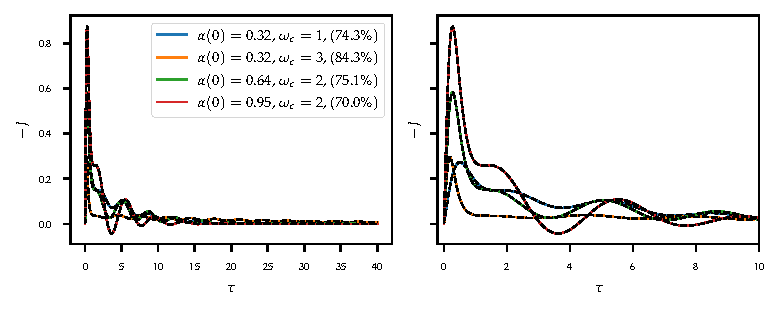
\includegraphics{figs/analytic_comp/flow_comp_zero.pdf}
  \caption{\label{fig:comp_zero_t} The bath energy flow \(-J\) for
    different parameters of the ohmic bath correlation function
    \cref{eq:ohmic_bcf}. The right panel shows the short time behaviour
    of the flow. The solid lines have been obtained with HOPS and the
    dashed lines using the analytic solution. A good agreement is
    evident visually and corroborated by the consistency values in the
    legend (see \cref{sec:meth} for an explanation).  The simulation
    with \(ω_{c}=3\) (orange) stands out for its slow long term decay,
    whereas the same simulation with longer bath correlation time
    (blue) initially decays much slower but falls below its orange
    counterpart for longer times.}
\end{figure}
\paragraph{Zero Temperature}
The bath energy flow \(J=-∂_t\ev{H_\bath}\), from here on called
simply ``the flow'' or ``bath energy flow'', for the zero temperature
case is plotted in \cref{fig:comp_zero_t}. The numerical results
(solid lines) agree with the analytical solutions (dashed lines) to a
very good accuracy, validating the findings of \cref{chap:flow}. For
all parameter choices the consistency is well above one standard
deviation.


The simulation was run with a hierarchy depth of
\(\norm{\vb{k}} \leq 5\) (simplex truncation\footnote{see
  \cref{sec:hops_basics}}) and a BCF fit with \(7\) terms taken from
\cite{RichardDiss} which was also used in the analytical solution. The
harmonic oscillator Hilbert space was truncated to \(15\) dimensions
in the energy basis. As the initial state the first excited state of
the oscillator was chosen so that some nontrivial energy flow would
occur. Some \(N=5000\) trajectories have been computed and lead to a
quite satisfactory statistical error that is small enough to be
invisible in \cref{fig:comp_zero_t}. The normalized standard deviation
of the bath energy flow follows the usual one-over-square-root rule as
is illustrated in \cref{fig:sqrt_conv}. Even after just \(N=1000\)
trajectories the normalized statistical error is on the order of
\(10^{-3}\).
\begin{figure}[htp]
  \centering
  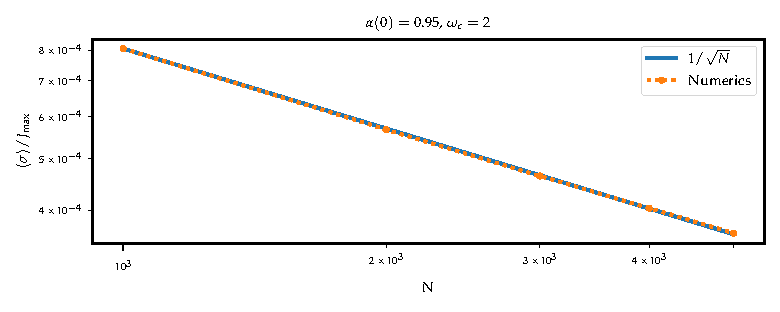
\includegraphics{figs/analytic_comp/sqrt_convergence.pdf}
  \caption{\label{fig:sqrt_conv} The (empirical) standard deviation
    (the statistical error) of the flow for the last configuration in
    \cref{fig:comp_zero_t} normalized by the maximum absolute value of
    \(J\). The \(1/\sqrt{N}\) rule is obeyed to good accuracy showing
    that the estimation of the variance is sound.}
\end{figure}
\begin{figure}[htp]
  \centering
  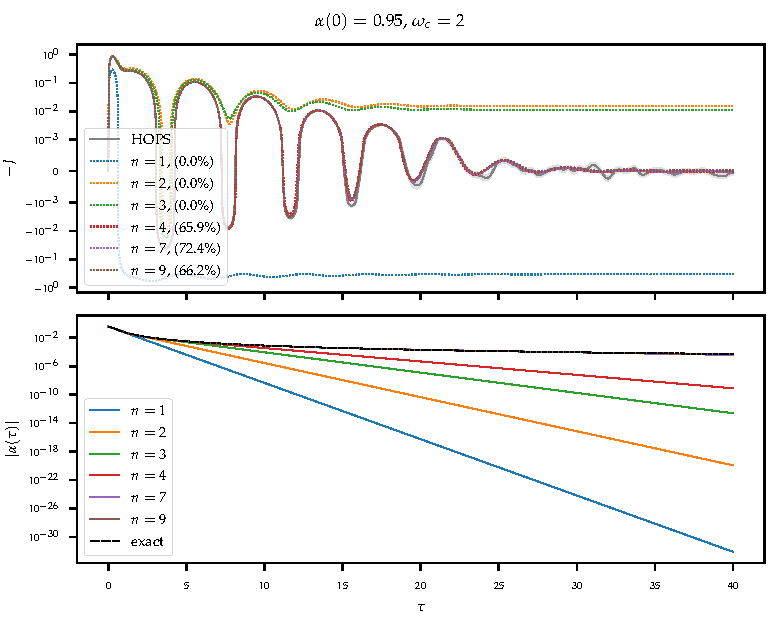
\includegraphics{figs/analytic_comp/analytical_terms_important.pdf}
  \caption{\label{fig:analytical_terms_important} Upper Panel: The
    analytical solution for the zero temperature bath energy flow
    using different numbers of terms in the BCF expansion in a
    symmetric logarithmic scale. For \(7\) terms the consistency
    (number in parentheses) with the numerical solution is best. For
    \(n<4\) the results are unphysical in the steady state.  Lower
    Panel: The absolute value of the approximated bath correlation
    function.}
\end{figure}

The analytical solution is quite sensitive to the quality of the BCF
expansion.  Despite choosing the same number of terms in the expansion
as in HOPS the simulation, there still remains a systematic difference
between HOPS and the analytical solution, as the stochastic processes
is sampled using the full bath correlation~\cite{RichardDiss}.
Nevertheless, the best agreement is found for using the same number
expansion terms in both HOPS and the analytical solution as is
illustrated in \cref{fig:analytical_terms_important}. Note that the
consistency value given in \cref{fig:analytical_terms_important} is
slightly different from the one in \cref{fig:comp_zero_t}, as here a
separate fit was made rather than using the fit from
\cite{RichardDiss}.

Interestingly, the solutions using a BCF expansion with three terms or
fewer lead to an unphysical non-zero steady state bath energy
flow. Considering specifically the case of one expansion term, this
may be related to the fact that now the BCF term so that
\(α(τ)=G \exp(-Wτ)\) is related to a Lorentzian spectral density that
also includes unphysical negative frequencies. To correctly reproduce
the steady state, the fit must model the decay of the BCF on the
appropriate time scales.

Although the simulations are primarily intended as a benchmark for
HOPS and a verification for the results of \cref{chap:flow} some
observations can be made in \cref{fig:comp_zero_t}.

First, the flows for different parameters all feature the
characteristic spike in the flow, not unlike an ``initial slip''. As
the initial state is a product state which is unaware of the
bath-system interaction, the state undergoes some short time dynamics
to compensate the change of the effective oscillator dynamics due to
the interactions~\cite{Weiss2012}.% As we shall see in
% \cref{sec:one_bath_cutoff}, the interaction energy is generally
% negative. The surge in bath energy and also the system energy (see
% \cref{fig:ho_zero_entropy}) compensates for this. We will find in
% \cref{sec:moder-init-slip} that this effect can be compensated, by
% activating the interaction in a more adiabatic way.

We will discuss this phenomenon further in \cref{sec:pure_deph} as it
is a quite universal feature and also shows up on a single trajectory
level, suggesting that it is not strictly related to an energy
exchange with the bath but rather to the build-up of interaction
energy. This will be discussed further in \cref{sec:one_bath_cutoff}.

Note that the model of \cref{sec:oneosc} used here is missing a
so-called counter term, which is often prescribed to obtain a stokes
like, velocity dependent friction term in the equations of motion and
takes the form \cite{Weiss2008Mar}
\begin{equation}
  \label{eq:counter_term}
  H_{\mathrm{C}} \sim ∑_{λ}\frac{\abs{g_{λ}}^{2}}{ω_{λ}} q^{2}.
\end{equation}
When \cref{eq:counter_term} is included in \cref{sec:oneosc}, our
model becomes the Caldiera-Legget Model.  The counter term balances
the renormalization of the system potential due to the bath. It is
therefore an interesting question how the initial slip behaves in its
presence.

The time dependence of the flow also varies both with the shape of the
BCF and the coupling strength. For longer correlation times
\(τ_{\bath}\propto 1/ω_c\) we find that the flow initially decays much
slower at the same coupling strength (blue and orange lines) and
exhibits stronger oscillations. After this initial period the
situation is reversed and the simulation cuttoff frequency \(ω_{c}=3\)
(orange line) exhibits prolonged oscillations. For large coupling
strengths we can observe a ``backflow'' of energy out of the bath as
can be observed for the red line in the right panel of
\cref{fig:comp_zero_t}. In all cases the flow features some
oscillations and decays to zero which is physical for the situation of
a harmonic oscillator that loses most of its energy into a zero
temperature bath.

When the bath memory is short however, the short-term energy flow is
of less magnitude. Correspondingly, the system energy decays slower
for shorter bath memories \cref{fig:ho_zero_entropy}. We will discuss
this point further in \cref{sec:one_bath_cutoff} in the context of
another model as the performance does not only depend on the bath
memory, but also on the concrete distribution of the spectral density
in frequency space.

\begin{figure}[htp]
  \centering
  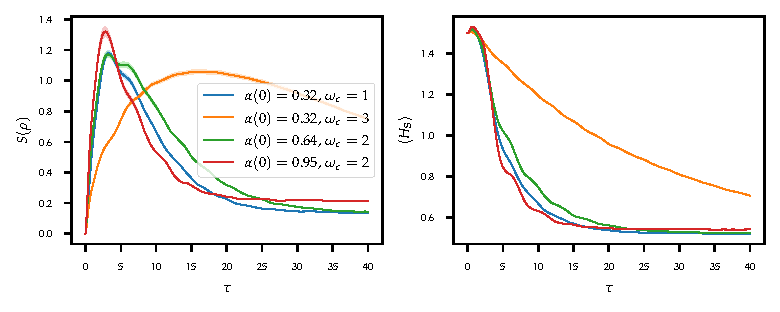
\includegraphics{figs/analytic_comp/entropy_zero.pdf}
  \caption{\label{fig:ho_zero_entropy} Left panel: The von Neumann
    entropy of the system state as a measure for entanglement with the
    bath. Right panel: The system energy as a function of time. The
    \(ω_{c}=3\) case (orange) is markedly different from the others,
    with a much slower decay of the system energy and slower entropy
    dynamics. The strongest coupling simulation (red) converges to a
    markedly different steady state.}
\end{figure}
The ``backflow'' observed in \cref{fig:comp_zero_t} for stronger
coupling seems to diminish the advantage of stronger coupling over
larger bath memories. The decay of the red curve in the right panel of
\cref{fig:ho_zero_entropy} is barely faster than the decay of the blue
curve, despite much larger coupling strength in the red case. This may
be due to the system interacting ``too long'' with a given portion of
the bath. Here we observe this behaviour for stronger coupling which
shortens the timescale of the energy exchange. In
\cref{sec:one_bath_cutoff} we will see, that these oscillations occur
generically for long bath memories and stronger coupling and how they
might be exploited.

Note also, that the steady state is not a product state as can be
determined from the residual entropy in \cref{fig:ho_zero_entropy} for
the cases where the steady state has been approximately
reached\footnote{Note that the global state is pure, so that the
  system state entropy is the correct measure of entanglement}. The
stronger the coupling, the larger the entanglement of system and bath
as measured by the system entropy. The simulation with coupling
strength \(α(0)=0.95\) (red line) appears to be leading to a
qualitatively different steady state than the one with the same cutoff
but weaker coupling strength (green line). This also manifests in a
higher expected system energy in the steady state.

\begin{wrapfigure}[18]{o}{0.4\textwidth}
  \centering
  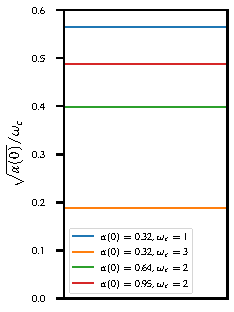
\includegraphics{figs/analytic_comp/timescale_comparison}
  \caption{\label{fig:timescale_comp} A comparison of bath vs
    interaction time scales
    \(\sqrt{α(0)}/ω_{c}\sim τ_{\bath}/τ_{\inter}\) for the simulations
    in \cref{fig:ho_zero_entropy}. The orange line is set far apart
    from the other simulations.}
\end{wrapfigure}
The time dependence of the entropy the expectation value of the system
energy is markedly different for the cutoff \(ω_c=3\) (orange
line). Although the coupling strength is similar to the
\(α(0)=0.32,\, ω_c=1\) case (blue line) the energy loss of the system
is much slower and the initial energy gain is less pronounced. This is
consistent with the flow in \cref{fig:comp_zero_t}. The case is set
apart by the long interaction timescale \(τ_{\inter}\) due to the
weaker coupling strength \(\sim α(0)^{-1/2}\) and the short bath
timescale \(τ_{\bath}\sim ω_{c}^{-1}\). Of course absolute values of
these time scales of no great value here. A comparison of relative
time scales \(\sqrt{α(0)}/ω_{c}\sim τ_{\bath}/τ_{\inter}\) can be
found in \cref{fig:timescale_comp} supporting the above argument.

\paragraph{Finite Temperature}
\begin{figure}[t]
  \centering
  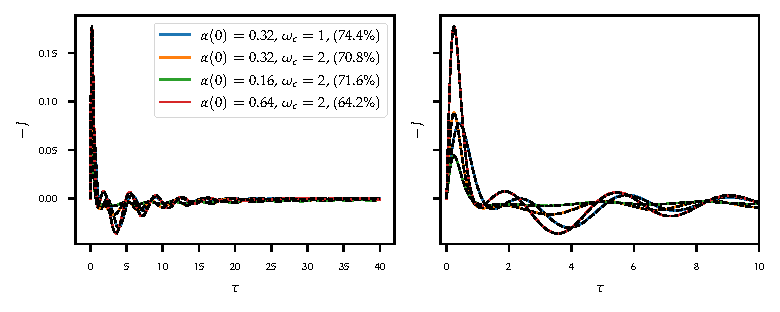
\includegraphics{figs/analytic_comp/flow_comp_nonzero.pdf}
  \caption{\label{fig:comp_finite_t} The bath energy flow \(-J\) of
    the quantum Brownian motion model for different parameters of the
    ohmic bath correlation function \cref{eq:ohmic_bcf} in the finite
    temperature \(T=1\) case. The presentation is equivalent to
    \cref{fig:comp_zero_t}.}
\end{figure}
The results for the finite temperature case are illustrated in
\cref{fig:comp_finite_t} for a temperature of \(T=1\). The setup was
otherwise equivalent to the zero temperature simulations, except for
the number of trajectories which was chosen to be \(N=10^5\) and the
initial state which was changed to the \(\ket{0}\) state.  Again the
high consistency values suggest that the findings of \cref{chap:flow}
are valid. The last case (\(α(0)=0.64,\, ω_c=2\), red line), falls
just short of the \(68\%\) mark, but agrees very well visually. It is
very probable that simply more samples are required.\fixme{maybe
  re-run...}

We find a similar behaviour to the zero temperature case, but this
time with a more pronounced flow (negative values in the plot) out of
the bath as it has a nonzero energy expectation value. For higher
coupling strengths, the flow amplitude is higher, as is also the case
for lower cutoffs.

One potentially contestable point in \cref{chap:flow} was the
appearance of the time derivative of the thermal stochastic process in
\cref{eq:pureagain}. The numerical method which is used to sample the
stochastic processes allows for a straight forward implementation of
this derivative so that no numerical derivatives are required and
there appears to be no problem.

As the dimensionality of the Monte Carlo integral underlying the
NMQSD/HOPS formalism is increased by the ``Stochastic Hamiltonian''
method, we observe markedly slower convergence as the variance of the
individual trajectories is higher. In \cref{fig:cons_dev_finite} the
convergence behaviour, as well the consistency with increasing
trajectory count are plotted and this symptom is observed. We also
find that in the more challenging regimes of stronger coupling or
longer bath correlation times the behaviour of the convergence is more
volatile, dipping into regions of inconsistency even at high sample
counts. While the mean difference between the numerical and the
analytical flow is always below the mean statistical error, larger
fluctuations can occur at certain points in time when a new region of
the probability space is sampled.

\begin{figure}[p]
  \centering
  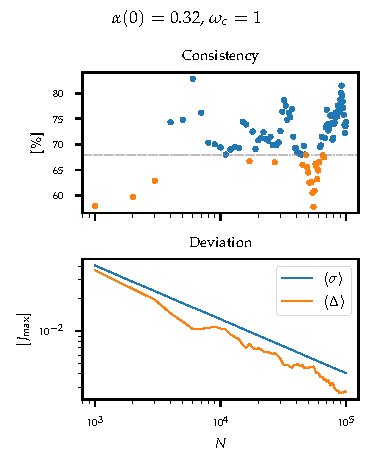
\includegraphics{figs/analytic_comp/consistency_development_0.pdf}
  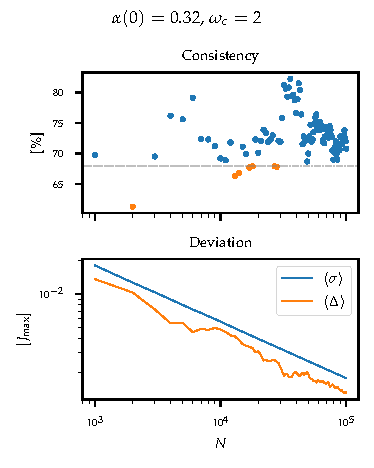
\includegraphics{figs/analytic_comp/consistency_development_1.pdf}
  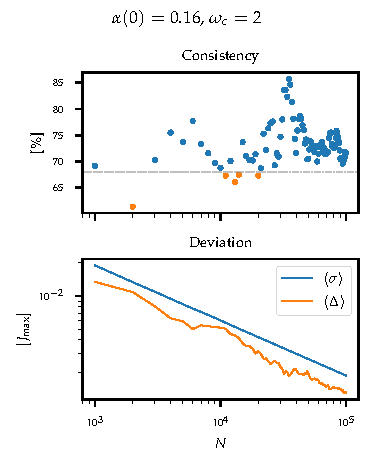
\includegraphics{figs/analytic_comp/consistency_development_2.pdf}
  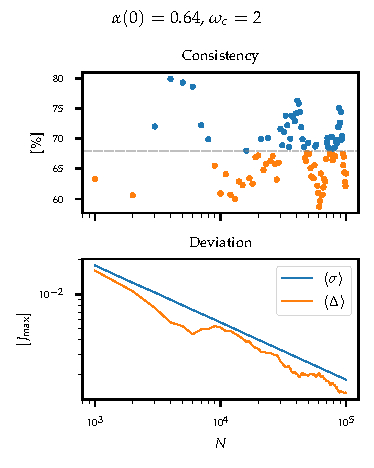
\includegraphics{figs/analytic_comp/consistency_development_3.pdf}
  \caption{\label{fig:cons_dev_finite} The convergence of the flows of
    \cref{fig:comp_finite_t} with increasing trajectory count. The
    upper panels show the consistency, where the grey line marks the
    \(68\%\) threshold for consistency. The lower panel shows the time
    averaged values of the statistical error \(\ev{σ}\) and the
    deviation from the analytical result \(\ev{Δ}\) normalized by the
    maximum absolute value \(J_{\mathrm{max}}\) of \(J\). In the last plot,
    the consistency development is quite unstable despite the mean
    deviation from the analytical result being smaller than the mean
    standard deviation. In all cases these two curves scale with the
    \(1/\sqrt{N}\) rule.}
\end{figure}

We have found, that we can expect precise numerical results for the
flow in the single bath case, both for zero and for finite
temperature. As systems with multiple baths are a different caliber,
both on the conceptual level, but also in the implementation of HOPS,
the method should also be verified for such settings. This will be
done in \cref{sec:twoosccomp}.
% The advantage of the ``Stochastic Hamiltonian'' method for finite
% temperature (see \cref{eq:thermalh}) is that one doesn't have to deal
% with the finite temperature BCF that does decay markedly slower than
% its zero temperature counterpart as is illustrated in
% \cref{fig:bcf_decay}. Generically, more terms in the BCF expansion
% would be required to capture the algebraic decay appropriately.

% \begin{figure}[t]
%   \centering
%   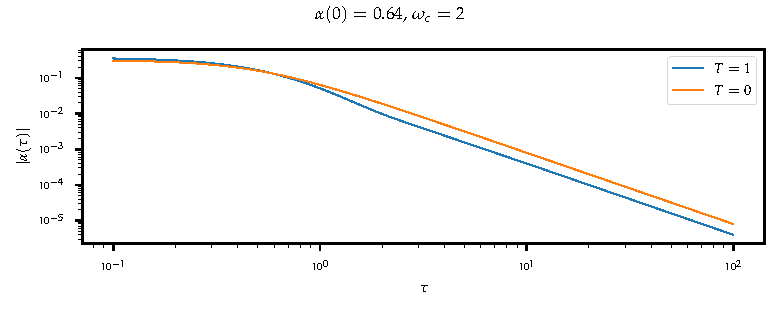
\includegraphics{figs/analytic_comp/bcf_decay.pdf}
%   \caption{\label{fig:bcf_decay} The absolute value of the Ohmic BCF
%     used in the last simulation of \cref{fig:comp_zero_t}.}
% \end{figure}

\subsection{Two coupled Harmonic Oscillators coupled to two Baths}
\label{sec:twoosccomp}
We now progress to a slightly more complicated setting, namely that of
two oscillators coupled to two baths\footnote{This also constitutes
  the first application of the TU-Dresden TQO group's HOPS code-base
  to multiple baths.}. As noted before, multiple baths are an
important ingredient for interesting models like quantum-thermodynamic
engines. At the same time, this setting is much more numerically
challenging as the number in BCF expansion terms doubles, which in
turn increases the number of hierarchy states.

The model of \cref{sec:oneosc} was generalized to two oscillators
coupled to two separate baths in \cref{sec:twoosc} and
\cref{eq:hamiltonian_two_bath}. In this section we simulate this model
and compare the results with the analytical solution.

For simplicity, the parameters were chosen symmetric so that the
frequencies of both oscillators are the same \(Ω=Λ=1\). As before,
\(Ω\) defines the energy unit. The zero temperature bath correlation
functions of both baths were chosen identically with a cutoff
frequency \(ω_c=2\). The intra-oscillator coupling was chosen as
\(γ=0.5\). The hierarchy was truncated so that \(\abs{\vb{k}}\leq 3\)
and a BCF expansion with five terms was chosen to limit memory demands
and \(10^{4}\) trajectories were integrated.

To limit the variance the temperature of one of the baths was set to
zero, so that only one thermal stochastic process was introduced. The
other bath was chosen to have \(T=0.6\). The ground state of the
system Hamiltonian \(\ket{0}\otimes \ket{0}\) was chosen as the
initial state of the oscillators.

The main challenge of simulating the model
\cref{eq:hamiltonian_two_bath} is the dimension of the system Hilbert
space which is constrained by the available memory. In the simulation
discussed here, each oscillator was truncated at \(9\) levels leading
to \(9^2 = 81\) dimensions in total\footnote{This is a naive method of
  truncation, but sufficient for the purposes of this work.}. The
effect of a too drastic truncation of the system Hilbert space can be
seen in \cref{fig:insufficient_levels}. At the temperature chosen, the
mean level occupation of a harmonic oscillator is given by the Bose
distribution
\begin{equation}
  \label{eq:harm_mean_occ}
  \ev{n} = \frac{1}{\eu^{Ωβ}-1} \approx 0.23 < 1.
\end{equation}
Nevertheless, quite more than two levels are required per
oscillator. This may be due to a required minimal resolution of the
position operators occurring in the model
\cref{eq:hamiltonian_two_bath} which is formulated with position space
in mind.

The final result can be studied in \cref{fig:sufficient_levels}. We
find good, but not excellent agreement. Based on the results of
\cref{sec:oneosccomp} however, it can be argued that this result is
sufficient to corroborate the validity of the results of
\cref{sec:multibath}. With more computational effort\footnote{Mainly
  more BCF expansion terms.} and fine-tuning of parameters an even
better agreement between the analytical and the numerical results may
be achieved.
\begin{figure}[htp]
  \centering
  \begin{subfigure}[t]{.49\linewidth}
    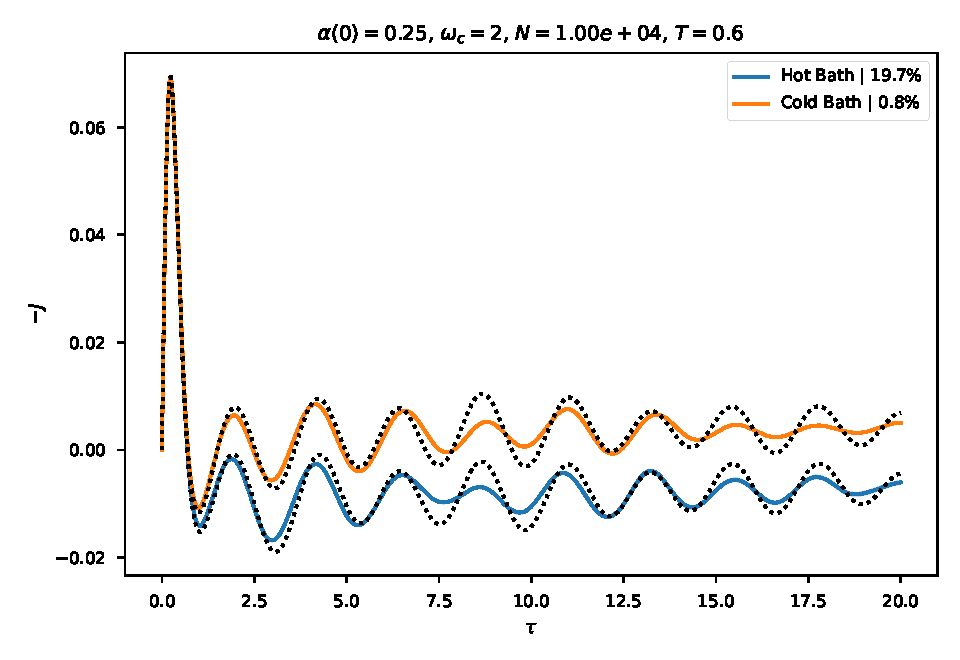
\includegraphics{figs/analytic_comp/comparison_two_5bcf_5ho.pdf}
    \caption{\label{fig:insufficient_levels}\(\dim\hilb_\sys=25\).}
  \end{subfigure}
  \begin{subfigure}[t]{.49\linewidth}
    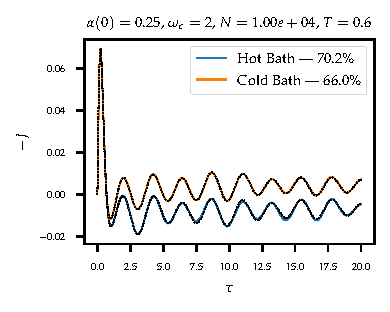
\includegraphics{figs/analytic_comp/comparison_two_ho.pdf}
    \caption{\label{fig:sufficient_levels}\(\dim\hilb_\sys=81\).}
  \end{subfigure}
  \caption{\label{fig:comp_two_bath} The bath energy flows for
    the model \cref{eq:hamiltonian_two_bath}, where the dashed lines
    correspond to the analytical solutions.}
\end{figure}

\Cref{fig:comp_two_bath} exhibits some interesting features. The
initial slip peak in the bath energy flows is identical for both baths
and independent of temperature as suggested by the discussion in
\cref{sec:pure_deph}. As is expected, the hot bath looses energy and
the cold bath gains energy, while this process is modulated by the
intra-oscillator coupling. It follows from the analytical solution
that eventually a steady state without oscillations will be reached.

The zero temperature bath flow converges very much faster than the
finite temperature flow despite the whole system being connected, at
least indirectly, to the hot bath. The reason for this is that the
derivative of the thermal stochastic process \(\dot{ξ}\) dominates the
variance of the flow for each trajectory. This is also the reason that
expressions depending on the hierarchy states rather than time
derivatives of stochastic processes are preferred as discussed in
\cref{sec:general_obs}.

We have shown that the findings of \cref{chap:flow} are consistent
with \cref{chap:analytsol} and that through a careful choice of the
HOPS parameters such as hierarchy depth, Hilbert space dimension and
BCF expansion the exact open system dynamics of the bath energy flow
can be reproduced. The statistical error can be made arbitrarily small
by increasing the trajectory count. For a given target error, the
required trajectory count can be estimated by the empirical standard
deviation of a given observable. In \cref{sec:pure_deph} we will
discuss the short term dynamics of our general model and explain the
peak in the flow, as seen in \cref{fig:comp_zero_t}.

For future work there remains the generalization of the work in this
section and \cref{chap:analytsol} to time dependent couplings and
Hamiltonians. Because the NMQSD and also HOPS are largely agnostic of
these factors, we may safely assume that the results of the comparison
will be similar to the ones presented here.

\section{Pure Dephasing and the Initial Slip}
\label{sec:pure_deph}
As seen in \cref{fig:comp_finite_t,fig:comp_zero_t,fig:comp_two_bath},
the short time behavior of the bath energy flow is dominated by
characteristic peak at short times. Because this peak occurs at very
short time scales, it may in part be explained by a simple calculation
which neglects the system dynamics by setting \(H_\sys=0\).

We solve the model with the Hamiltonian (Schr\"odinger picture)
\begin{equation}
  \label{eq:puredeph}
  H = L^†(t) B + L(t) B^† + H_\bath
\end{equation}
with \(L(t)=L(t)^†\), \([L(t), L(s)] = 0\;\forall t,s\) (so that
Heisenberg Hamiltonian matches \cref{eq:puredeph}) and \(B,\,H_\bath\)
as in \cref{sec:nmqsd_basics}.

Because \([L,H]=0\) we can immediately solve \(L_H(t)=L_S(t)\), where
the subscript distinguishes the Heisenberg and Schr\"odinger pictures
respectively. The Heisenberg equations for the \(a_λ\) yield
\begin{equation}
  \label{eq:alapuredeph}
  a_λ(t) = a_λ(0) \eu^{-\iu ω_λ  t} - \iu g_λ^\ast∫_0^t\dd{s} L(s)
  \eu^{-\iu ω_λ  (t-s)}.
\end{equation}

This allows us to calculate
\begin{equation}
  \label{eq:pureflow}
  \dot{H}_\bath =\iu\comm{H_{\inter}}{H_{\bath}} = - ∑_λ g_λ L(t) \qty[∂_t a_λ(0) \eu^{-\iu ω_λ t} - \iu
  g_λ^\ast∫_0^t\dd{s} L(s) ∂_t \eu^{-\iu ω_λ (t-s)}] + \hc,
\end{equation}
which gives with a state of the form \(ρ=\ketbra{ψ} \otimes ρ_β\)
(\(ρ_β\) being a thermal state of inverse temperature \(β\))
\begin{equation}
  \label{eq:pureflowexpectation}
  \ev{\dot{H}_\bath } = -2 ∫_0^t\dd{s}\ev{L(t)L(s)} \Im[\dot{α}(t-s)].
\end{equation}
For time independent \(L\) this becomes
\begin{equation}
  \label{eq:pureflowtimeindep}
  \ev{\dot{H}_\bath } = -2 \ev{L^2} \Im[α(t)].
\end{equation}

The proportionality to the imaginary BCF \(α\) does explain the
initial peak in the bath energy flow. The imaginary part of the BCF is
zero for \(t=0\) and then usually features a peak at rather short
times (assuming finite correlation times). For the ohmic BCF used here
and shown in \cref{fig:ohm_bcf_ex}, this feature is very prominent.
\begin{figure}[htp]
  \centering
  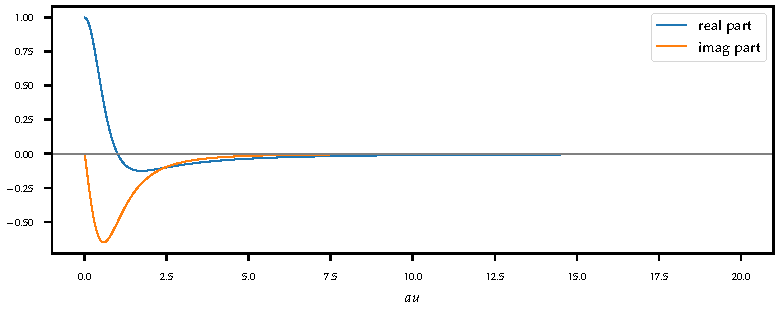
\includegraphics{figs/misc/ohmic_bcf_example.pdf}
  \caption{\label{fig:ohm_bcf_ex} An ohmic BCF with \(ω_{c}=η=1\). The
  imaginary part has a peak at the beginning and decays to zero.}
\end{figure}

Generically, the imaginary part of the BCF is negative at least for
short times as it takes the form
\begin{equation}
  \label{eq:negtive_imag}
  \Im[α(τ)] = -\frac{1}{π}∫_{0}^{τ}J(ω) \sin(ωτ)\dd{ω}
\end{equation}
which is negative for \(τ\leq π/ω_{\mathrm{max}}\), where
\(ω_{\mathrm{max}}\) is a characteristic cutoff frequency of the
system. The direction of the initial slip flow for unmodulated systems
will therefore be always be into the bath compensating for negative
interaction energy.

Interestingly, \cref{eq:pureflowexpectation} does not contain any
reference to the temperature of the bath. Therefore, the bath energy
can only surpass its initial value in this model, as the dynamics
match the zero temperature case in which the bath has minimal energy
in the initial state.

A thermodynamically useful model should feature significant system
dynamics which is always given assuming that the coupling is no too
strong. Coupling that is not self-adjoint \fixme{plot: if time, i
  could do the energy shovel with non-hermitian} may also have this
effect, but in the literature most effective qubit models tend to
favour Hermitian couplings
\cite{Aurell2019Apr,Hita-Perez2021Nov,Hita-Perez2021Aug,MacQuarrie2020Sep,Andersen2017Feb,Mezzacapo2014Jul}. For
the spin-boson model, non Hermitian coupling it is the result of the
rotating wave approximation assuming that system and bath scales are
quite different, which however does not imply weak
coupling~\cite{Irish2007Oct}.

For completeness, the interaction energy is given by
\begin{equation}
  \label{eq:pureinter}
  H_\inter = L(t)\qty[∑_λg_λ\qty(a_λ(0)\eu^{-\i ω_λ t} - \i
  g^\ast_λ∫_0^t\dd{s} L(s) \eu^{-\i ω_λ (t-s)})] + \hc,
\end{equation}
yielding
\begin{equation}
  \label{eq:pureinterexp}
  \ev{H_\inter} = 2 ∫_0^t\dd{s}\ev{L(t)L(s)} \Im[α(t-s)].
\end{equation}

For time independent coupling we have
\begin{equation}
  \label{eq:pureinterexp_timeidp}
  \ev{H_\inter} = 2 \ev{L^2} \int_{0}^{t}\Im[{α}(s)]\dd{s} = -Δ\ev{H_{\bath}}.
\end{equation}

It may be useful to normalize the BCF based on \cref{eq:pureinterexp},
so that the pure interaction energy build-up in the initial slip is
taken as measure of interaction strength. To make the normalization
independent of \(L(t)\), we choose the normalization to be
\begin{equation}
  \label{eq:bcfnorm}
  \begin{aligned}
  \mathcal{N} &= 2 \abs{\frac{\max_t\norm{L(t)L^\dag(t)+\hc}}{\max_t{\norm{H(t)}}} ∫_0^∞ \Im[α_u(τ)]\dd{τ}}\\
    α(τ) &= α_u(τ)/\mathcal{N},
  \end{aligned}
\end{equation}
where \(α_u\) is some unnormalized BCF. This normalization has the
useful property, that it neutralizes any scaling in \(L\). Note that
here the convention in which \(α\) is dimensionless is used.

% this is not true
% imaginary part becomes proportional to the Dirac delta in the limit
% where typical cutoff frequency \(ω_c\rightarrow ∞\). The integral over
% the real part of \(α\) always gives zero if the spectral density obeys
% \(J(0) = 0\) and tends to exhibit fast oscillations and fast decay in
% the large-cutoff limit. For weak coupling, it may therefore be
% neglected. This constitutes the Markov limit mentioned in
% \cite{Strunz2001Habil}.
The Ohmic-type BCF is
\begin{equation}
  \label{eq:normohmic}
  α(τ)=\frac{ω_c  s }{ (\max_t\norm{H})(1+\iu ω_c τ)^{s+1}},
\end{equation}
in this normalization.

After this brief detour we will again concentrate on the numerical
aspects and the phenomenology of the energy flow of the spin-boson
model in \cref{sec:prec_sim}.

\section{Precision Simulations of the Zero Temperature Spin-Boson Model}
\label{sec:prec_sim}
Despite being soluble analytically, the models from
\cref{sec:hopsvsanalyt} are numerically cumbersome, as their system
Hilbert space is infinite dimensional and has to be truncated. In this
section we concern ourselves with a very simple model that poses
lesser numerical challenges and still exhibits interesting behaviour.

Both the performance of the HOPS method itself
(\cref{sec:stocproc,sec:trunc}) and the characteristics of the flow
mediated by the concrete form of the bath correlation function
(\cref{sec:one_bath_cutoff,sec:one_bathcoup_strength}) will be
investigated. We will find that the numerics do indeed yield very
consistent results and that the specifics of the energy flow depend
very much on the spectral density.

As an analytical solution to a given open system is generally not
known, another indicator of the proper choice of HOPS parameters is
required. Upon the example of a single qubit coupled to a single zero
temperature bath, we will study the convergence behaviour of the
interaction energy.  The corresponding Hamiltonian is
\begin{equation}
  \label{eq:one_qubit_model}
  H = \frac{1}{2} σ_z + \frac{1}{2} ∑_λ\qty(g_λ σ_x^† a_λ + g_λ^\ast
  σ_x a_λ^†) + ∑_λ ω_λ a_λ^\dag a_λ,
\end{equation}
where we have chosen \(H\) to be dimensionless.

In the language of HOPS this corresponds to \(H_\sys=σ_z/2\),
\(L=σ_x/2\). We again choose the Ohmic BCF as explained in
\cref{sec:meth}. Throughout this section we choose the ``up'' state
\(H_S\ket{1} = 1/2\ket{1}\) as the initial state of the system.

The main measure of convergence for variables other than the
trajectory count are consistency conditions. One check available to us
is energy conservation, which allows us to calculate the expectation
value of the interaction energy through integration of the bath energy
flow. The interaction energy obtained in this way can then be compared
to the interaction energy obtained directly as shown in
\cref{sec:intener}. Note that this scheme may also be adapted easily
to multiple baths where the sum of interaction energies has to be
considered and to time dependent Hamiltonians where finite power has
to be taken into account.

Sources of systematic deviations for the model
\cref{eq:one_qubit_model} are the quality of the sampling of the
stochastic process and the truncation of the hierarchy. The first
becomes important when the cutoff frequency is large and the BCF
vanishes rapidly necessitating it to be resolved on shorter time
scales. The hierarchy truncation is important when the cutoff
frequency is smaller and the bath has a longer memory.

\subsection{Stochastic Process}
\label{sec:stocproc}
For studying the convergence behaviour regarding the sampling of the
stochastic process we chose the cutoff \(\norm{\vb{k}} \leq 4\)
(simplex truncation\footnote{see \cref{sec:hops_basics}}),
\(N=4.5 \cdot 10^5\) trajectories and an Ohmic BCF with \(α(0)=1.6\)
and \(ω_c=4\).  The sampling method uses the ``Fast Fourier
Transform'' (FFT) as described in~\cite{RichardDiss}. As the system
Hilbert space dimension is small, a BCF expansion with seven terms was
employed~\cite{Hartmann2021Aug,RichardDiss}.

The main parameter of this method is the accuracy of the FFT. The
implementation compares the BCF and its FFT approximation on the time
interval of the simulation to choose the internal
parameters\footnote{The number of time grid points and the integral
  boundaries in frequency space.} so that the difference normalized by
\(α(0)\) of the FFT transformed spectral density and the exact BCF is
smaller than a given value \(ς\).

\begin{figure}[htp]
  \centering
  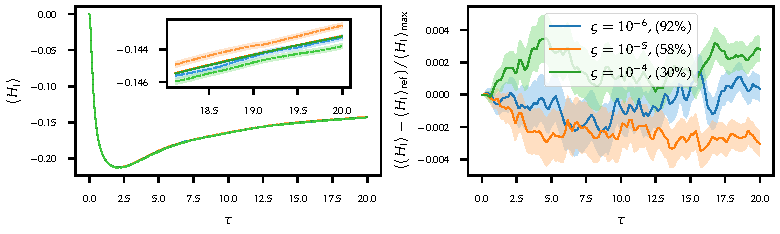
\includegraphics{figs/one_bath_syst/stocproc_systematics_interaction}
  \caption{\label{fig:stocproc_systematics} Left panel: The
    interaction energy of the model \cref{eq:one_qubit_model} for
    \(α(0)=1.6\) and \(ω_c=4\) using different precisions for the
    sampling of the stochastic process. The dashed lines are obtained
    using energy conservation while the solid lines are obtained
    directly as in \cref{sec:intener}. The consistency between the two
    is given in the legend of the right panel. An inset shows the
    curves for the final three time units. Right panel: The difference
    of the interaction energies obtained using energy conservation and
    directly. The values are normalized by the maximal absolute value
    of the interaction energy. The \(\varsigma = 10^{-6}\) case gives
    the most accurate results in terms of energy conservation, but
    when using the direct method of calculating \(\ev{H_{\inter}}\)
    all parameter choices yield the same results.}
\end{figure}
\Cref{fig:stocproc_systematics} illustrates the effect of this
parameter. We find very good qualitative agreement for all values of
\(ς\). The indirectly calculated value (dashed lines) of the
interaction energy shows some fluctuation between the settings, but
the value calculated directly (solid lines) is very stable as can be
seen in the inset of \Cref{fig:stocproc_systematics}.

Only in the case with precision \(\varsigma=10^{-6}\) (blue) however,
compatibility is satisfied at the given sample count. This is due to
the fact that here multiple values that are obtained in different
ways, namely system energy and the flow. The system energy can be
calculated directly from the system state whereas the flow has to be
numerically integrated to obtain the total bath energy change.
\begin{figure}[htp]
  \centering
  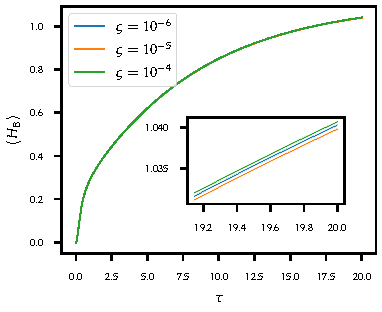
\includegraphics{figs/one_bath_syst/stocproc_systematics_bath_energy}
  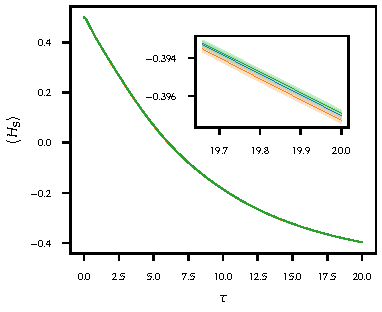
\includegraphics{figs/one_bath_syst/stocproc_systematics_system}
  \caption{\label{fig:stocproc_bath_sys}The bath and system energies of the
    model \cref{eq:one_qubit_model} for \(α(0)=1.6\) and \(ω_c=4\)
    using different precisions \(\varsigma\) for the sampling of the
    stochastic process. Systematic deviations outside the error bounds
  occur mainly in the bath energy.}
\end{figure}

The individual contributions to the indirectly obtained interaction
energy may be studied in \cref{fig:stocproc_bath_sys}. The bath energy
\(\ev{H_{\bath}}\), being an integrated quantity for which errors
accumulate, is most susceptible to systematic deviations outside the
error bounds, as is clearly visible in the insets. Nevertheless, the
qualitative agreement of the different simulations is excellent.

The development of the consistency over the trajectory count \(N\) is
plotted in \cref{fig:stocproc_consistency_dev}. Only for the highest
precision (blue) case good consistency is given continually. For lower
precision (green, orange), the consistency fluctuates and only
occasionally surpasses \(68\%\). Initially compatibility is being
demonstrated (until about \(N=10^4\)) but a divergence diverge from
the most precise\footnote{The result that demonstrates compatibility
  consistently.} result occurs. It is therefore important to consider
the dependence of the compatibility on the sample count \(N\) to judge
the veracity of the simulation results.
\begin{figure}[htp]
  \centering
  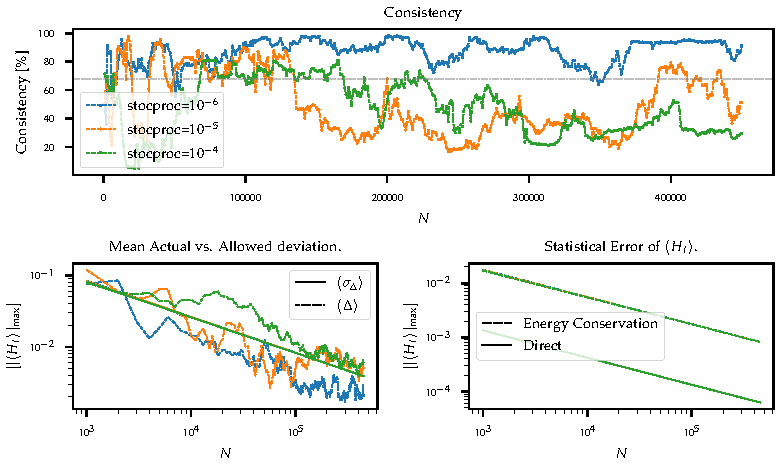
\includegraphics{figs/one_bath_syst/stocproc_systematics_consistency}
  \caption{\label{fig:stocproc_consistency_dev} Upper panel: The
    compatibility (number of values within one standard deviation of
    other, see \cref{sec:meth}) of the flow (direct computation
    vs. energy conservation) of the model \cref{eq:one_qubit_model}
    for \(α(0)=1.6\) and \(ω_c=4\) using different precisions
    \(\varsigma\) for the sampling of the stochastic process in
    relation to the trajectory count \(N\). Only the
    \(\varsigma=10^{-6}\) simulation is consistent for all sample
    counts. Lower left: The time averaged difference of the direct and
    indirect interaction energies (dashed) and the time averaged
    standard deviation of the difference (solid) as a function of
    trajectory count. Only for the smallest \(\varsigma\) the
    difference is consistently smaller than the standard deviation of
    the difference. Lower right: The time averaged statistical errors
    of the interaction energy calculated directly (solid lines) and
    indirectly through energy conservation (dashed lines). The
    deviation of the direct method smaller by an order of magnitude.}
\end{figure}

Apart from being closer to the correct result, the direct computation
of the interaction energy has the advantage of providing faster
convergence as demonstrated in \cref{fig:stocproc_consistency_dev}.

\subsection{Hierarchy Truncation}
\label{sec:trunc}
As the effect truncation depth has already been studied thoroughly
in~\cite{RichardDiss}, we will keep the discussion short.  We chose
\(N=4.5 \cdot 10^5\) trajectories and an Ohmic BCF with \(α(0)=0.8\)
and \(ω_c=2\). Again, seven a BCF expansion with seven terms have been
used. The coupling strength has been chosen with the help of
\cref{sec:pure_deph}, so that the interaction energy is of a similar
order of magnitude as in the discussion
above. \Cref{fig:k_systematics} suggests that there seems to be no
improvement in accuracy or even change in the value of the flow for
\(\norm{\vb{k}}\geq 4\). However, the inset in the left panel
demonstrates that the direct result differs slightly for
\(\norm{\vb{k}} = 2\), which demonstrates that an adequate choice of
truncation depth is important.
\begin{figure}[htp]
  \centering
  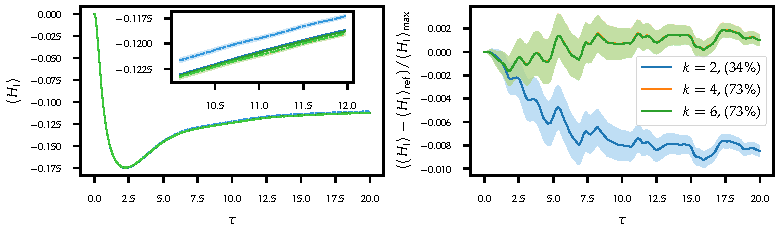
\includegraphics{figs/one_bath_syst/k_systematics_interaction}
  \caption{\label{fig:k_systematics} The same as
    \cref{fig:stocproc_systematics} but for \(α(0)=0.8\) and
    \(ω_c=2\) and for various truncation depths \(k=\norm{\vb{k}}_{\mathrm{max}}\).}
\end{figure}


We see in \cref{fig:k_systematics_system} that the difference of the
\(\norm{\vb{k}} = 2\) (blue lines) case from the \(\norm{\vb{k}} = 6\)
is on the same order of magnitude for system energy (solid line) and
interaction energy (dashed line). The bath energy (dotted line), being
an integrated quantity, accumulates errors and deviates the
most. Also, the results for \(\norm{\vb{k}} = 4,6\) (orange line)
agree perfectly in all cases.
\begin{figure}[htp]
  \centering
  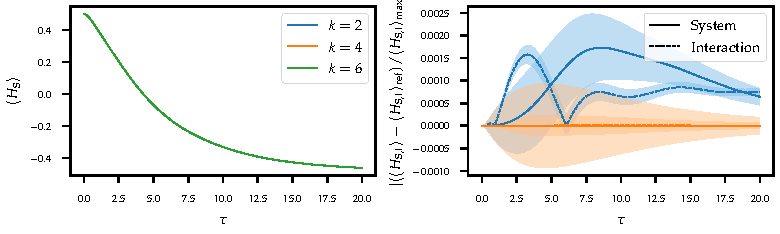
\includegraphics{figs/one_bath_syst/k_systematics_system}
  \caption{\label{fig:k_systematics_system} Left panel: The norm of
    the difference of a single trajectory to the \(\norm{\vb{k}} = 6\)
    case. The solid lines show the difference of the zeroth hierarchy
    states and the dashed lines show the same for the first hierarchy
    states.  There is still a slight difference on the trajectory
    level. Right panel: The difference between the \(k=6\) result and
    the results with \(k<6\) normalized by the maximal absolute system
    energy (solid lines) and the same for the interaction energy
    (dashed lines) as well as the bath energy change (dotted). The
    deviation is most substantial for the bath energy change, as
    errors can accumulate in the integration of the bath energy flow.}
\end{figure}
The left panel of \cref{fig:k_systematics_system} demonstrates, that
there is still a difference greater than the machine epsilon on the
level the trajectories. This difference however, is small enough not
to impact observables much.

Summarizing, we conclude that the HOPS parameters have to be chosen
carefully for precision simulations, but that a more relaxed choice of
parameters already give a \emph{very} good qualitative picture
depending on the observable. Numerical integration should be avoided
where possible.

\fixme{maybe run a simulation with more hierarchy depth and more bcf
  terms, check whether there is a mistake} It remains for future work
to perform a detailed study of the systematics of the finite
temperature flow and modulated Hamiltonians. In the following sections
we will look at some examples of physically interesting systems with
less focus on the systematics of convergence.

\subsection{Varying the Cutoff Frequency}
\label{sec:one_bath_cutoff}
The lessons learned in \cref{sec:stocproc,sec:trunc} will now be
applied to simulate \cref{eq:one_qubit_model} with high consistency
for various parameter choices of the cutoff \(ω_{c}\) of the Ohminc
BCF (see \cref{sec:meth})
\begin{equation}
  \label{eq:ohmic_bcf_repeat}
  α(τ) =
  \frac{η}{π}\qty(\frac{ω_c}{1+\iu ω_c τ})^2.
\end{equation}
Guided by these demonstrations, we'll turn to a more detailed analysis
of the role of non-Markovianity in the energy transfer characteristics
of our model. The quantification of the initial slip dynamics in
\cref{sec:pure_deph} will also be verified.

To make the interaction energies comparable to each other, the BCF
normalization of \cref{sec:pure_deph} is being used. Because
of the small size of the Hilbert space, we were able to choose a HOPS
configuration\footnote{\(\norm{\vb{k}}\leq 7\), seven BCF terms,
  \(\varsigma = 10^{-6}\)} that yields high-accuracy
results\footnote{A detailed account of the consistency is given in
  \cref{fig:omega_interaction_consistency}.}, based on the results of
the previous section. The only problematic result is the one for cutoff
\(ω_c=1\), but there is good qualitative consistency in this case.

For all simulations \(N=5\cdot 10^{5}\) trajectories were integrated
to produce the results that are summarized in
\cref{fig:omega_systematics_system}.
\begin{figure}[htp]
  \centering
  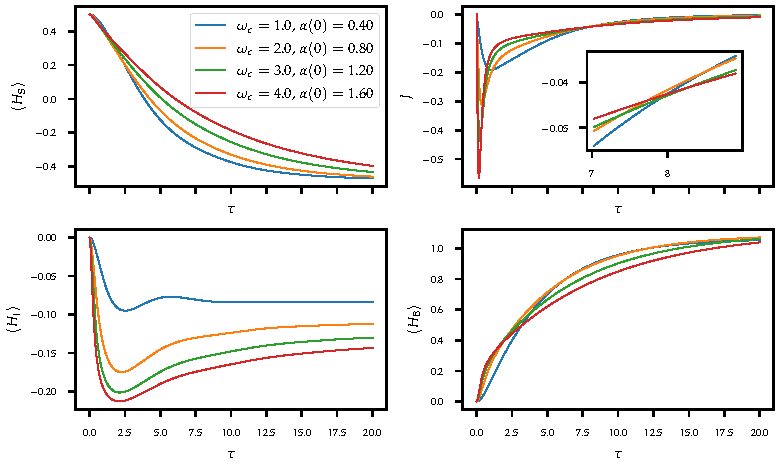
\includegraphics{figs/one_bath_syst/omega_energy_overview}
  \caption{\label{fig:omega_systematics_system} Energy overview for the
    model \cref{eq:one_qubit_model} for various coupling strengths and
     cutoff frequencies. The curves are converged, and the error
    funnels are not visible.}
\end{figure}

Let us preface the following discussion with a note of caution. All
the discussed phenomena are specific to the minimal model
\cref{eq:one_qubit_model}, although sometimes similarities to
phenomena observed in \cref{sec:hopsvsanalyt} can be seen. Whether
there is some universality to the results obtained is an interesting
question for a more detailed future detailed study.\fixme{Remove this?}

The interaction energy expectation values, despite being in the same
order of magnitude and not in the weak coupling regime, differ
significantly. This illustrates the limitation of the estimate in
\cref{sec:pure_deph} and exemplifies the nontriviality of the open
system dynamics. Better estimates of the interaction energy and thus
interaction strength may be derived from ideas similar to the ones
discussed in \cref{sec:normest}.  Besides the magnitude, the
qualitative time dependence of the interaction energies varies,
especially between the configuration with the cuoff frequency
\(ω_c=1\) (blue) and the others.

The curve with the cuoff frequency \(ω_c=1\) (blue) exhibits two
pronounced turning points in contrast to the other simulations. This
behaviour is a symptom of the very long bath memory, as we will
discuss below. Further, despite having the weakest overall coupling
strength \(α(0)=0.4\) the system energy falls off the fastest after a
short period where it is above the other configurations. This
behaviour is also visible in the bath energy expectation value, where
this simulation almost reaches the same levels as the \(ω_c=2\)
configuration (orange) for \(τ\gtrsim 5\).

The flow is generally negative (the bath gains energy) and decays
after an initial peak. All the flow graphs appear to be crossing in
about the same point \(τ\approx 7.7\) after which their ordering by
magnitude is reversed.  The inset shows that the crossing is not
precisely at the same point, nevertheless further investigation of
this phenomenon may of interest in the future.  Due to the pure
dephasing behavior discussed in \cref{sec:pure_deph}, a greater cutoff
coupled with a greater coupling strengths leads to a higher peak in
the flow for short times. After the peak the flow decays the faster,
the higher the cutoff. The situation is reversed after some time so
that the flow of higher cutoffs decays slower.  This is due to the
fact that still more system energy is left to be transmitted to the
bath.

The presentation in \cref{fig:omega_systematics_system} is not
conducive to comparing the actual performance of the energy transfer,
due to the variable shape of the spectral density and the chosen
coupling strengths. Because the maximum of the Ohmic spectral density
is located at \(ω_c\), the special observed energy transfer behaviour
for \(ω_c=1\) is likely due to a resonance effect (see above) as the
system energy level spacing is unity.

The dissipator of the master equation for this two level system only
depends on the value of the spectral density at the level
spacing~\cite[p. 66]{Rivas2012}\footnote{There \(L=σ_{+}\), but this
  has no bearing on the connection to \(ω_{0}\).}  (\(ω_{0}=1\) here),
so that it is reasonable to expect, that there may be variations
whenever its magnitude at this point changes.  On the other hand, a
strong dependence of the flow on the shape of the bath correlation
function beyond lamb-shift like influences, as we will find below, is
an indicator of the departure from the weak coupling limit.
\fixme{Here, some master equation comparison would be nice.}

\subsection{Energy Transfer Characteristics}
\label{sec:energy-transf-char}
After focusing on the systematics and achieving very high consistency
in our simulations, we continue to shed some light on the role of bath
memory and resonance between system and bath in the behaviour of the
energy transfer between system and bath.

\begin{wrapfigure}{o}{0.3\textwidth}*
  \centering
  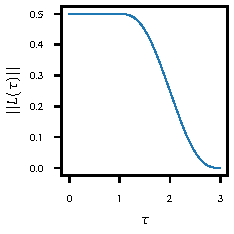
\includegraphics{figs/one_bath_syst/L_mod}
  \caption{\label{fig:L_mod} The smooth modulation of the coupling
    operator \(L(τ)\).}
\end{wrapfigure}
For a systematic study of resonance, we first compare the flow for
shifted ohmic spectral densities\footnote{See \cref{sec:shift_sp} for
  details.} with identical scaling \(α(0)\) and cutoff frequency
\(ω_c=2\). We turn off the interaction smoothly\footnote{A smoothstep
  function of order two with a transition period of two. See
  \cref{sec:smoothstep}.} over two time units before the system has
reached its steady state and compare how much energy has been
transferred in terms of the final bath
\(\ev{H_{\bath}}\)\footnote{This is actually a slight misnomer, as we
  consider the \emph{change} of bath energy. The bath energy itself is
  infinite.} and system energies and the total energy change
\(Δ\ev{H}\) due to the modulated coupling.

The less energy the system has at the end of the process and the
faster the process concludes, the better the performance of
transfer. If the interaction energies are on the same scale, the
decoupling costs should be roughly the same in terms of total energy
change. Otherwise, they may lead to an additional change of system and
bath energies between the different simulations. Ideally the bath
energy changes to take up any energy introduced into the system by the
decoupling rather than the system energy.

To make space for the shifted bath correlation functions in frequency
space, the system energy gap has been set to the value four so that
\(α(0)=8\) represents a quite reasonable coupling strength for our
purposes here.

The results for three shifts are presented in
\cref{fig:resonance_analysis}. For all shifts the spectral density has
a finite value at the value of system level spacing, but only in the
case with the cutoff \(ω_s=2\) (orange), the resonance condition is
fulfilled. Indeed, the energy transfer out of the system is the best
for the resonant case (see \cref{fig:resonance_analysis}, middle
panel), as the final system energy is the lowest.

The change in total energy due to the decoupling of the bath is
moderately higher than in the resonant (orange) case than for cutoff
\(ω_s=1\) (blue) and seems to be somewhat proportional to the
interaction energy which is reasonable. The decoupling process appears
to affect the bath energy curves in this case. As can be gathered from
\cref{fig:resonance_analysis}, the bath energies generally decreases
when decoupling, compensating for the negative interaction energy. The
effect on the system energy is masked by the much greater energy loss
to the bath.

Were the interaction switched off abruptly, the system and bath
energies would remain untouched. Turning the interaction off in finite
time reduces the energy introduced into the system in the cases
discussed here. System and bath energy must therefore compensate part
of the negative interaction energy when the system is decoupled from
the bath. Hence, the observed lowering the bath energy after
decoupling. However the effect can also act into the other direction
as we shall see below.
\begin{figure}[htp]
  \centering
  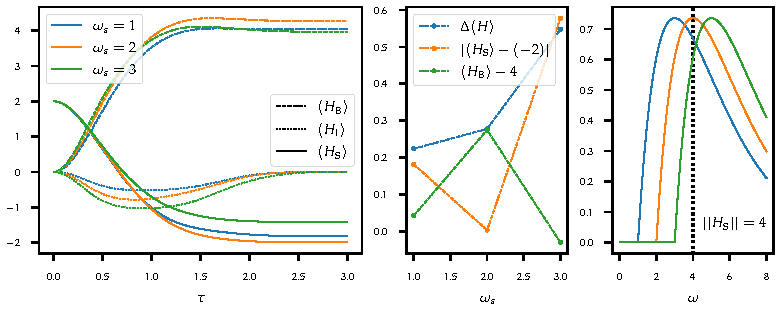
\includegraphics{figs/one_bath_syst/resonance_analysis}
  \caption{\label{fig:resonance_analysis} Left
    panel: The system, bath and interaction energies for various Ohmic
    BFCs with \(α(0)=8,\,ω_c=2\) shifted by \(ω_s\). Mid panel: The
    difference in total energy, the distance of the system energy to
    the ground state energy and the distance of the bath energy to the
    initial system energy. Right panel: The spectral density for the
    three shift values. \(\norm{H_\sys}\) does mean in this case, that
    the energy level spacing of the system is \(4\). There resonant
    case has the best energy transfer behaviour as gauged by the final
    system energy.}
\end{figure}

The third simulation with cutoff \(ω_s=3\) (green) exhibits the worst
energy transfer with the highest residual system energy and the
highest change in total energy due the large magnitude of the
interaction energy.  The lowering of the final bath is most pronounced
as the interaction energy is largest. As very much energy is shed into
interaction initially, the bath energy can't decay as much as in the
situation with cutoff \(ω_{s}=1\) (blue).


Due to the asymmetry of the spectral density, the simulations for
\(ω_s=1\) and \(ω_s=3\) are not directly comparable. A repetition of
this investigation with a (pseudo~\cite{Mukherjee2020Jan}) Lorentzian
spectral density and for different interaction
time-frames\footnote{steady state vs. transient states} is left for
future work.

Interestingly, if we modulate the system periodically with angular
frequency \(Δ\), also bath frequencies of \(ω_{0} + n Δ\)
(\(n\in\NN\)) become important, so that shifting the spectral density
to higher frequencies is advantageous, albeit for the completely
different objective of extracting energy from system and bath, as we
will find out in \cref{sec:modcoup_reso}.

% Turning of the interaction leads mostly to a reduction of the final
% bath energy (see the middle panel).  This effect will also appear in
% most of the cases discussed below. When deriving a master equation for
% this two level system~\cite[p. 68]{Rivas2012}, there occurs a lamb
% shift term that acts as a correction to the unitary evolution of the
% system. Turning the interaction off adiabatically removes this leads
% to a change in what one may define as system energy in this case. In
% the case discussed here, the coupling is not weak so that this
% explanation may only serve as a means of analogy. Compensating for the
% negative interaction energy, the system and bath energy expectation
% value both fall when the coupling is turned off.\fixme{is this
%   reasonable?}

% For an ohmic spectral density the lamb shift energy is
% \begin{equation}
%   \label{eq:lshift_twolevel}
%   2Δ=\eu^{-1/ω_{c}}\,\mathrm{Ei}\qty(\frac{1}{ω_{c}}) - ω_{c},
% \end{equation}
% which is negative for all the cases discussed here and may account for
% some part of the negative interaction energy. In this way, the removal
% of the bath would

\begin{wrapfigure}[-1]{O}{0.4\textwidth}*
  \centering
  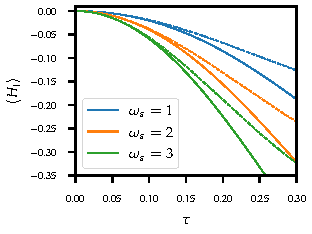
\includegraphics{figs/one_bath_syst/initial_slip_resonance}
  \caption{\label{fig:initial_slip_resonance} The interaction energies
    (solid lines) of the models in \cref{fig:resonance_analysis} and
    the predictions for the interaction energy due to the initial slip
    dynamics \cref{eq:pureinterexp_timeidp} (dashed lines). Larger
    frequency shifts of the spectral density lead to a higher
    magnitude of the interaction energy and faster dynamics.}
\end{wrapfigure}
In general, the maximal absolute interaction energy is roughly
proportional to the shift \(ω_{s}\) of the spectral density, so that
the short term interaction strength as measured by the interaction
energy expectation value is not only dependent on the width and total
norm of the spectral density, but also on its absolute distribution in
frequency space. The shift adds a phase factor \(\eu^{-\i ω_{s} τ}\)
to the BCF which makes the imaginary part steeper for short
times. This in turn leads to faster initial slip dynamics and a speeds
up buildup of interaction energy as demonstrated in
\cref{fig:initial_slip_resonance}. The observed effect is sensible on
an intuitive level as higher frequency oscillators are being excited
in the bath leading to faster dynamics.

The longer term picture is being studied in
\cref{fig:resonance_analysis_steady}. We see broadly similar energy
transfer characteristics for the cutoffs \(ω_{s}=1\) (solid blue line)
and \(ω_{s}=2\) (solid orange line), where the off-resonant case
(blue) may be slightly advantageous. The left panel shows, that
although the system energy before the decoupling is lower in the
resonant case (orange), the situation is reversed during the
decoupling as now also the system energy is affected by the modulation
and the interaction energy of the off-resonant case is slightly larger
in magnitude. However these effects are quite marginal and should be
taken with care. The system energy difference amounts to
\(\Delta\langle H_\mathrm{S}\rangle=0.00397\pm 0.00010\), but only the
statistical error has been taken into account. The simulations were
run with \(N=10^{4}\) trajectories and the same HOPS settings as in
the discussion above, so that some confidence may be placed in them.

For \(ω_{s}=3\) (green lines) the approximate steady state has not
been reached yet and the energy transfer is incomplete so that the
residual system energy is the highest. As remarked earlier, th fast
growth of the interaction energy leads to a slower initial loss of
system energy. On longer time scales we see a slow, almost linear
transfer of energy from the system (solid line) into the interaction
(dotted line). The system dynamics are catching up with the bath.
\begin{figure}[htp]
  \centering
  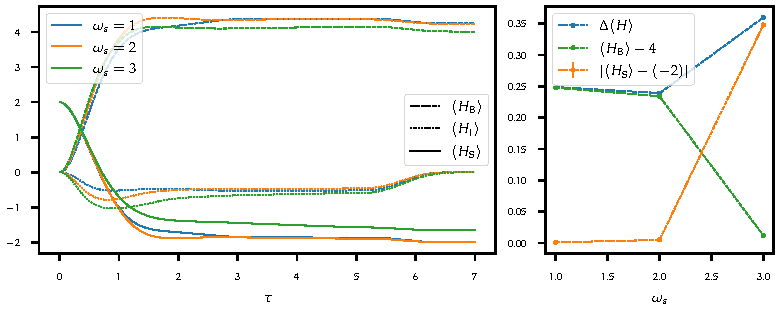
\includegraphics{figs/one_bath_syst/resonance_analysis_steady}
  \caption{\label{fig:resonance_analysis_steady} The same as
    \cref{fig:resonance_analysis} but for a longer coupling time.}
\end{figure}

Let us now turn to the impact of non-Markovianity on the energy
transfer into the bath.  To study the effect of the bath memory, we
use Ohmic spectral densities with linearly spaced
\(τ_{\bath}\equiv ω_c^{-1}\) that have been shifted and scaled by
numerical optimization so that their peaks coincide and the resulting
maximal absolute interaction energies identical. The rightmost panel
of \Cref{fig:markov_analysis} shows plots of the spectral densities
obtained. We can see, that not only the magnitude at resonance point
enters, as the peak heights are quite different. We will encounter
this behavior again in \cref{sec:extr_mem}\footnote{Performing the
  optimization in the weak coupling regime will actually yield
  matching peak heights for the spectral densities.}.

The results that can be obtained are very much dependent on the time
when the interaction is switched off. \Cref{fig:markov_analysis} has
been arrived at by tweaking the time point of decoupling so that an
extremum in the system energy of the long memory (\(τ_{B}=1\)) case
(green) is captured. This leads to an advantageous transfer
performance with a lower system energy and similar cost in terms of
total energy change, although residual system energy is still higher
than in \cref{fig:resonance_analysis_steady}.  Despite the system
energy initially fall off the fastest for the short memory case (blue)
the situation is reversed after about \(τ=0.5\).
\cref{fig:resonance_analysis_steady}.
\begin{figure}[htp]
  \centering
  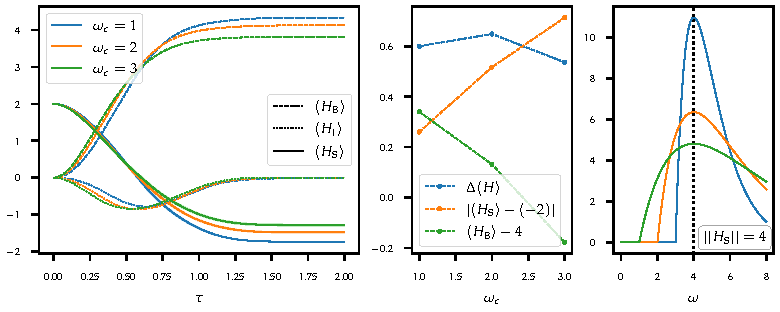
\includegraphics{figs/one_bath_syst/markov_analysis}
  \caption{\label{fig:markov_analysis} The same as
    \cref{fig:resonance_analysis} but for shifted spectral densities
    various bath memory times. The long-memory case performs best in
    this case, exhibiting the lowest final system energy.}
\end{figure}

Because the minimum in the interaction energy of the case with bath
memory \(τ_{\bath}=1\) (green) comes last, the residual interaction
energy and thus interaction strength is strongest when the interaction
is turned off. Therefore the largest quantity of energy is being
introduced into the system in this case when the interaction is
disabled. In all cases the amount of energy introduced is so large,
that the bath energy slightly rises during the decoupling process
instead of falling as in \cref{fig:resonance_analysis_steady}.


\begin{figure}[htp]
  \centering
  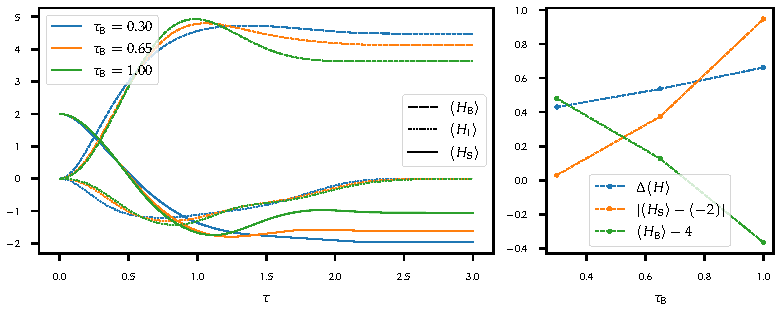
\includegraphics{figs/one_bath_syst/markov_analysis_longer}
  \caption{\label{fig:markov_analysis_longer} The same as
    \cref{fig:markov_analysis} but with slightly different timing. The
    result is exactly the reverse of
    \cref{fig:markov_analysis_longer}. Longer memories perform worse.}
\end{figure}
For slightly longer coupling times but with the same coupling
strengths, we find in the exact opposite picture as can be ascertained
from \Cref{fig:markov_analysis_longer}.  The increased bath memory
time allows for ``back flow'' of energy from the bath into the system
(blue and orange solid lines) and thus the performance of energy
transfer is strongly dependent on the precision of control. The
oscillations of flow and thus bath energy have already been noticed in
\cref{sec:oneosccomp} and seem to be a robust feature of stronger
coupling and long bath memories.

The total energy introduced is slightly less than in the earlier
simulation as the interaction energy is lower when the interaction is
switched off. The final bath energies show an inverse behavior,
falling as the final system energies rise. This is due to the similar
total energy change \(Δ\ev{H}\) in all three cases (blue line, right
panel). Such behavior can also be observed \cref{fig:markov_analysis}.

For even longer times we find in \cref{fig:markov_analysis_steady} a
picture similar to \cref{fig:markov_analysis_longer}. The short memory
case (blue) exhibits hardly any backflow and performs best in terms of
final system energy which is extremely close to the target value of
negative two. The other two bath memories perform worse (green,
orange). We observe that simulation with the longest bath memory
\(τ_{\bath}=1\) (green) stands out and having a very different final
state as is exemplified by the final system energy and the interaction
energy curve which exhibits a greater magnitude and persistent
oscillations. These oscillations were not clearly visible in the
earlier simulations
(\cref{fig:markov_analysis,fig:markov_analysis_longer}) due to the
modulation of the interaction. Because of the long memory the bath,
interaction and, to a lesser extend, the system can continue to
exchange energy, even in the steady state. We will encounter them
again in a different setting in \cref{sec:extr_mem}.
\begin{figure}[htp]
  \centering
  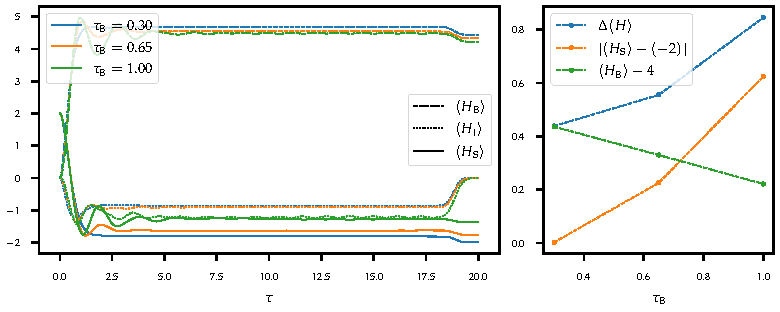
\includegraphics{figs/one_bath_syst/markov_analysis_steady}
  \caption{\label{fig:markov_analysis_steady} The same as
    \cref{fig:markov_analysis} but for long times. The results are
    broadly similar to \cref{fig:markov_analysis_longer} with the
    \(τ_{\bath}=1\) case standing out.}
\end{figure}

In the two simulations with shorter memory (blue and orange lines) we
find that about half of the interaction energy is compensated by the
total energy change. The rest is accounted for by a lowering of system
and bath energy alike, an effect that is strongest in the short memory
case especially for the system energy. A slower, more adiabatic
coupling modulation could likely further reduce the amount of energy
introduced.

That the steady state system energies\footnote{Before the interaction is
  switched off.} are greater than the ground state energy of the
system in all simulations of \cref{fig:markov_analysis_steady} is a
token of strong coupling. The ground state of the two level system is
not the steady state, as it would be with GKSL
dynamics~\cite{Binder2018}.

We have often alluded to the fact that oscillations in the system
energy, the back-flow of energy into the system, are a token of
departure from the Markovian regime. An explicit demonstration of this
fact is given in \cref{fig:steady_relent}.

Spohn's theorem~\cite{Breuer2002Jun} states that the negative time
derivative of the relative entropy of system state and steady state
must be positive if the dynamics are generated by GKSL dynamics.
In mathematical terms Spohn's theorem can be formulated as
\begin{equation}
  \label{eq:spohn}
  -\dv{\qrelent{ρ_{\sys}(t)}{ρ_{\sys}(∞)}}{t} \geq 0,
\end{equation}
where \(\qrelent{ρ}{σ}=\tr[ρ \log_{2} ρ - ρ \log_{2} σ]\) is the
quantum relative entropy. The left hand side of \cref{eq:spohn} is
called entropy production.
\begin{figure}[htp]
  \centering
  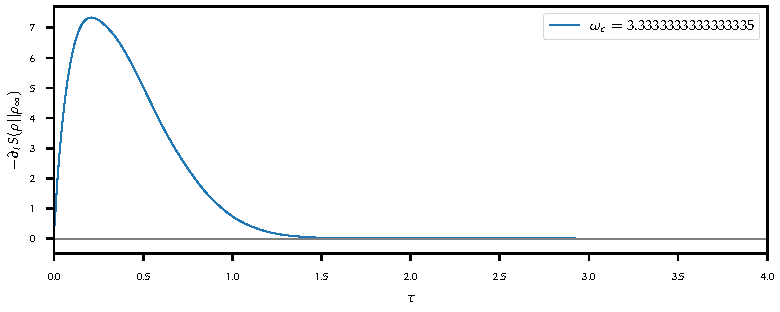
\includegraphics{figs/one_bath_syst/steady_relent}
  \caption{\label{fig:steady_relent} The negative time derivative of
    the relative entropy of system state and the approximate steady
    state (before the interaction is switched off) of the simulations shown in
    \cref{fig:markov_analysis_steady}. The short memory case does not
    violate Spohn's inequality, but the other two cases do. Note
    however, that the \(τ_{\bath}=1\) case has not yet reached a
    steady state and should therefore be treated with care.}
\end{figure}

\Cref{fig:steady_relent} demonstrates that the two simulations with
longer bathe memories are inconsistent with Markovian dynamics, as
their entropy production exhibits strong negativity. The
\(τ_{\bath}=1\) must be taken with care, as the steady state exhibits
oscillations. Then again, those are token of non Markovianity
themselves, as \cref{eq:spohn} forbids them.

The enhanced short term energy transfer for long bath memories may be
understood qualitatively through the NMQSD equation.%   Let \(τ^{\ast}\)
% be the time in which the BCF decays sufficiently and \(τ\) be some
% point in time with \(τ>τ^{\ast}\). The NMQSD equation
% \cref{eq:nmqsd_single} features two terms that model the interaction
% with the bath. The driving term
% \begin{equation}
%   \label{eq:nmqsd_driving}
%   L {η}^\ast_t\ket{ψ({η}^\ast_t, t)}
% \end{equation}
% includes the bath memory in an indirect manner through the stochastic
% process \(η^\ast\). At the time point \(τ\), the process will be
% effectively uncorrelated with itself at \(τ-τ^\ast\). Increasing
% \(τ^\ast\) will make the fluctuations of \(η^\ast\) slower and reduce
% their magnitude as demonstrated in \cref{fig:stocproc_comparison}.
% This allows for steadier dynamics with a slower bath induced change in
% the trajectory and state.
% % This in turn reduces the fluctuations of the bath energy flow on a
% % trajectory level and allows for steadier accumulation.  This effect
% % may be best understood by looking at the alternative expression for
% % the flow \cref{eq:alternative}
% % \(\dot{η}_t^\ast \mel{\psi(η,t)}{L}{\psi(η^\ast,t)}\), which features
% % the derivative of this process directly.

% The memory term
% \begin{equation}
%   \label{eq:nmqsd_memory_term}
%   L^†∫_0^τ\dd{s}α(t-s)\fdv{\ket{ψ({η}^\ast_t, t)}}{η^\ast_s}
% \end{equation}
% contains the bath correlation time even more explicitly. One may
% choose the integration range in \cref{eq:nmqsd_memory_term} to be
% \((τ-τ^\ast, τ)\) in good approximation due to the decay of the
% BCF. Thus, the evolution of the trajectory is not being directly
% influenced by times before \(τ-τ^\ast\). Also, if the stochastic
% process fluctuates more slowly, the trajectory has a stronger
% dependence on its past values, enhancing the magnitude of the
% functional derivative.  We see therefore, that the memory time of the
% bath has a very direct influence on the dependence of the trajectory
% and therefore system dynamics on its earlier states.

The memory term
\begin{equation}
  \label{eq:nmqsd_memory_term}
  L^†∫_0^τ\dd{s}α(t-s)\fdv{\ket{ψ({η}^\ast_t, t)}}{η^\ast_s}
\end{equation}
creates an explicit dependence of the system dynamics on earlier
states and connects the bath memory encoded in the BCF \(α\) with the
actual dynamics. The longer the bath memory is, the smoother is the
stochastic process \(η_{t}^\ast\) and the greater is the influence of
the memory term. These facts can be observed in
\cref{fig:memory_term,fig:stocproc_comparison}, where it is clearly
visible that a greater bath memory time \(τ_{\bath}\) leads to a
greater influence of the memory term and smoother processes.
\begin{figure}[htp]
  \centering
  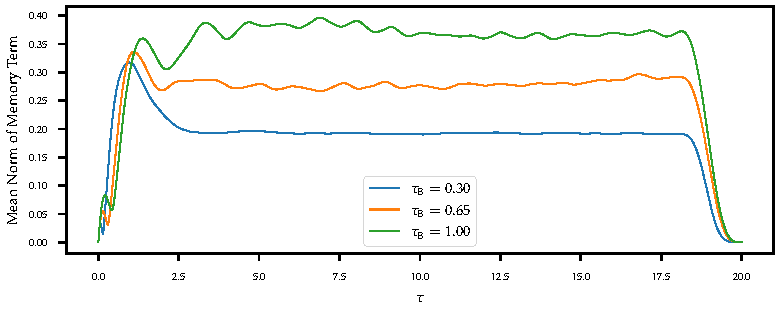
\includegraphics{figs/one_bath_syst/memory_term}
  \caption{\label{fig:memory_term} The norm of the memory term
    \cref{eq:nmqsd_memory_term} averaged over \(N=500\)
    trajectories. The longer the bath memory \(τ_{\bath}\), the
    greater the influence of the memory term.}
\end{figure}

As the memory is mediated by the bath degrees of freedom, a
dependence on ever earlier system states must be due to ever longer
interaction with specific bath degrees of freedom.

This interpretation is corroborated by the time discrete version of
the NMQSD discussed in \cite{RichardDiss}. There, the
\emph{Time-Oscillator picture} is introduced, which shows that the
NMQSD can be formulated as the successive interaction in time of the
system with mode like degrees of freedom. At each time point, a new
oscillator is being coupled to the system and the coupling to the
existing oscillators is weakened according to the bath correlation
function.

With this in mind, we may conclude that because we interact for a
longer time with certain ``portions'' of the bath degrees of freedom,
the energy exchange between the bath and the system can be more rapid,
as the energy exchange with the individual modes becomes more
complete.  At the same time, energy may flow back into the system from
those degrees of freedom if the bath memory is sufficiently long. On
the other hand, energy can only be lost to a zero temperature bath
when the memory is short.

In summary, we find that the energy dynamics of system, interaction and
bath depend strongly on the characteristics of the bath.  In the
regime studied, optimizing for fast energy loss of the system favors
longer bath memories, whereas the situation is reversed when longer
coupling times are allowed.

A resonance phenomenon has been observed which is already present in
the weak coupling case. However, here we additionally found a strong
dependence of the dynamics upon the shape of the whole spectral
density.

Note that the short time behaviour discussed here can usually not be
resolved by GKSL dynamics. This is due to the fact, that the bath
timescale \(\sim 1/ω_{c}\) must be by far the shortest
timescale. Another demonstration of this fact is given in
\cite{Link2022Feb}, where Markovian dynamics are compared with the
Redfield and exact dynamics for the spin-boson model coupled to a
squeezed bath. As in \cite{Xu2022Mar}, the Redfield description is
found to be adequate for weak coupling. This is due to the fact, that
the Redfield master equation does not require the secular
approximation, but only weak coupling and can therefore capture
non-Markovian dynamics.

We discussed the short term dynamics for a general model in
\cref{sec:pure_deph}.  Now, in \cref{sec:initial-slip-sb} we will
apply them the spin-boson model.

\subsection{Initial Slip}%
\label{sec:initial-slip-sb}
\begin{figure}[htp]
  \centering
  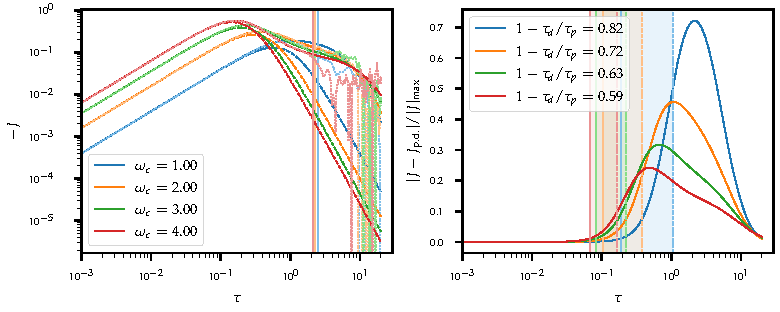
\includegraphics{figs/one_bath_syst/omega_initial_slip}
  \caption{\label{fig:omega_initial_slip} Left panel: The bath energy
    flow of the model \cref{eq:one_qubit_model} for various coupling
    strengths (solid lines) and the pure dephasing flow of
    \cref{sec:pure_deph} (dashed lines). The dotted lines show the
    flow calculated from one trajectory and the vertical lines mark
    the position of the peak of the absolute value of the interaction
    energy. Right panel: The difference of the actual flow \(J\) and
    the pure dephasing flow \(J_\mathrm{p.d.}\). The solid vertical
    lines mark the time \(τ_p\) where the normalized deviation from
    pure dephasing is \(10^{-2}\) and the dashed vertical lines show
    the position of the peak flow at time \(τ_p\). The divergence from
    pure dephasing dynamics occurs before the peak flow and the
    earlier the longer the bath memory. The single trajectory flow
    matches the converged flow for a longer period.}
\end{figure}

As the initial peak in the energy flow is also very prominent in the
simulations in this chapter, we return to
\cref{fig:omega_systematics_system} and compare the dynamics of those
simulations to the pure dephasing case of \cref{sec:pure_deph}. A good
agreement for short times is to be expected, as the system can't take
up energy in its initial state (up), so that all of the interaction
energy must initially be compensated solely by the bath.

We see in \cref{fig:omega_initial_slip} that the pure dephasing
dynamics (dashed lines) are accurate for very short time scales, but
fail to predict the correct location of the peaks in the absolute
value of the exact bath energy flow (solid lines).  The deviation
occurs before the peak, where the time difference between the peak and
the deviation increases with increasing bath memory \(\propto 1/ω_c\),
as does the magnitude of the maximal normalized deviation (right
panel). This can be ascertained from the legend of
\cref{fig:omega_initial_slip} where the difference between deviation
and peak time normalized by peak time is given.

We can conclude that for longer bath memory along with weaker
coupling, the role of the system Hamiltonian dynamics in modulating
the flow becomes increasingly important as now the system dynamics
happen on the same time scale as the bath dynamics and the
approximation \(H_{\sys}\approx 0\) is increasingly invalid.

The flow calculated from a single trajectory (dotted lines in
\cref{fig:omega_initial_slip}) matches the converged flow longer than
the pure dephasing approximation. For large cutoffs \(ω_{c}\) (green
and red) the single trajectory even matches until after the peak flow,
whereas the deviation occurs earlier for the \(ω_{c}=1\) case
(blue). The stochastic nature of the single trajectory dynamics seems
to become important only after a finite amount of time, longer than
period of pure dephasing dynamics.

For short times the flow is mainly influenced by the buildup of the
auxiliary states rather than the fluctuations of the stochastic
process, leading to a similar behavior for most trajectories.  This is
very useful, as this period of rapid dynamics must be resolved very
precisely to accurately integrate the flow into the bath energy
change.  \Cref{fig:flow_buildup} illustrates this phenomenon. The mean
norm of the auxiliary states (blue solid line) deviates from its
single-trajectory equivalent (orange dashed line) at the same time as the
mean flow (green solid line) deviates from the single trajectory flow
(red dashed line).
\begin{figure}[htp]
  \centering
  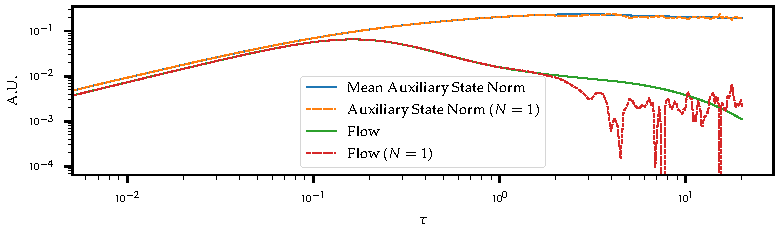
\includegraphics{figs/one_bath_syst/flow_buildup}
  \caption{\label{fig:flow_buildup} The total norm of the first
    auxiliary states and the flow for one trajectory and as a mean
    over all trajectories for the \(ω_{c}=4\) simulation. For short
    times the results for one trajectory match the ensemble means. The
    divergence between one trajectory and the mean occurs at
    roughly the same time for the flow and the auxiliary state
    norm. Moreover, flow and mean auxiliary state norm have the same
    functional form for very short times, apart from a scaling
    factor. The initial dynamics are therefore mainly concerned with
    populating the auxiliary states.}
\end{figure}

\Cref{sec:pure_deph} also treated time dependent coupling which we
haven not encountered so far. The effect of modulating the coupling
upon the bath energy change due to the initial slip, is the subject of
\cref{sec:moder-init-slip}.


\subsection{Moderating the Inital Slip with Modulated Coupling}%
\label{sec:moder-init-slip}
\begin{wrapfigure}[-1]{O}{0.4\textwidth}*
  \centering
  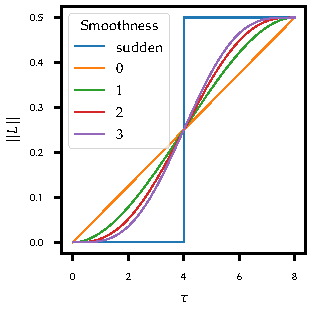
\includegraphics{figs/one_bath_mod/modulation_protocols_init.pdf}
  \caption{\label{fig:L_mod_init} The interaction is being switched on
    smoothly over a period of \(8\) time units by the use of
    smoothstep functions (\cref{sec:smoothstep}) of different
    orders. A sudden protocol is being included for reference.}
\end{wrapfigure}
In \cref{sec:pure_deph} we derived the short term behavior of the
interaction dynamics by neglecting the system Hamiltonian. Up to now
we only have looked at the scenario in which the interaction is
present from the beginning. Now we will briefly demonstrate a case
where the interaction is switched on smoothly as in
\cref{fig:L_mod_init}.

The model is otherwise the same as \cref{eq:one_qubit_model}, where we
have chosen \(α(0)=1.6\) and \(ω_{c}=1\) for all the simulations. Some
\(N=10^{4}\) trajectories have been computed for each simulation.

The smoothness parameter \(s\) regulates to which order the derivative
of the modulation is continuous at \(t=0\) and \(t=8\). The modulation
of the coupling allows for a change in total energy. This leads to a
partial compensation for the ``initial slip'' of the bath.

\begin{figure}[htp]
  \centering
  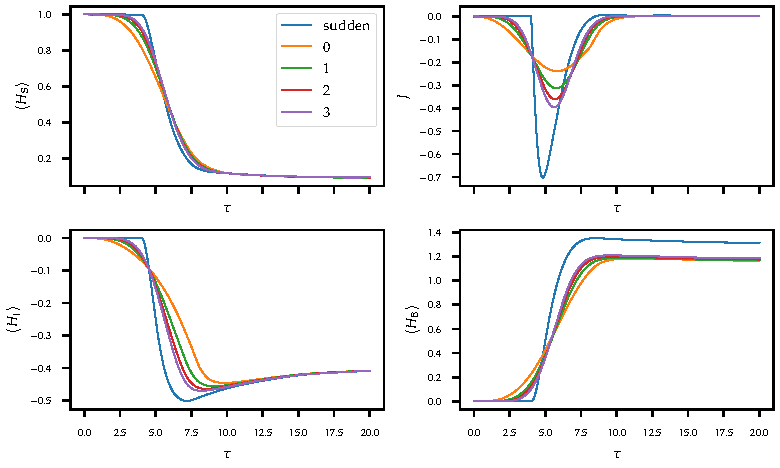
\includegraphics{figs/one_bath_mod/init_overview}
  \caption{\label{fig:init_energies}The relevant energy quantities for
    the different modulation protocols.}
\end{figure}
An overview over the bath system and interaction energy, as well as
the bath energy flow can be found in \cref{fig:init_energies}. System
\(\ev{H_{\sys}}\) and interaction energy \(\ev{H_{\inter}}\) all
converge to the same values after some time, but the flows \(J\) and
bath energies are the greater, the faster we switch the coupling
on. The sudden switching of the interaction (blue) is the extreme case
set apart by much greater interaction energies and a greater final
bath energy, as well as a much steeper initial peak in the flow.

The simulation with smoothness zero (yellow) exhibits a clear kink in
the bath energy flow and interaction energy curves at the time point
\(τ=8\), which reflects the lack of smoothness of the first derivative
of the modulation.

\cref{fig:init_total} shows that modulation protocols with a shallower
slope lead to a greater change in the total energy, compensating for
the negative interaction energy and leading to a shallower initial
slip flow. Activating the coupling adiabatically will likely lead to a
complete avoidance of the initial slip. On the other hand, the system
and interaction dynamics will be intermingled increasingly with the
interaction buildup.

An interesting future application would be to simulate an adiabatic
transition from the non-interacting ground state into the interacting
ground state and a study of energy released in this way, especially
for strong coupling.

The initial slip flow \cref{eq:pureflowexpectation} is valid for short
times.  \Cref{fig:init_slip_mod} demonstrates that the qualitative
properties of the flow are still being capture quite well for short
times. The actual flow (solid lines) and the pure dephasing flow
(dashed lines) agree initially but diverge quite some time before peak
flow.
\begin{figure}[htp]
  \centering
  \begin{subfigure}[t]{0.49\linewidth}
    \centering\captionsetup{width=.8\linewidth}
    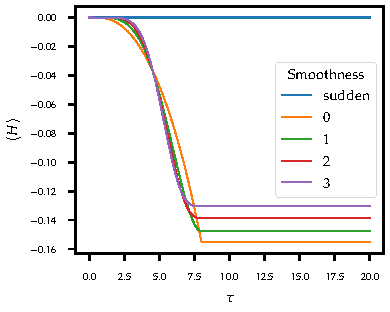
\includegraphics{figs/one_bath_mod/total_init}
    \caption{\label{fig:init_total}The total energy for different
      modulations. The slower the modulation, the more energy is
      released and the less energy is gained by the bath (see
      \cref{fig:init_energies}).}
  \end{subfigure}%
  \begin{subfigure}[t]{0.49\linewidth}
    \centering\captionsetup{width=.8\linewidth}
    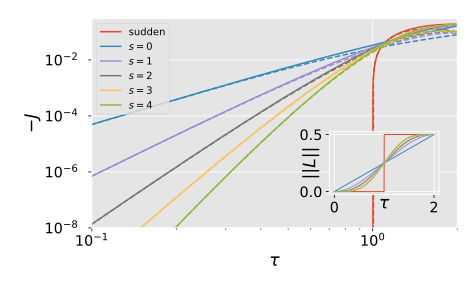
\includegraphics{figs/one_bath_mod/initial_slip_modcoup}
    \caption{\label{fig:init_slip_mod} The initial slip flow of
      \cref{eq:pureflowexpectation} and the exact flow. Initially, the
      flows coincidence, validating the earlier result. The flow peak
      heights and positions are being predicted incorrectly, but the
      initial slope and magnitude ordering are correct.}
  \end{subfigure}
  \caption{Total energy and flow for different interaction switching
    protocols.}
\end{figure}


Let us now complete our precision studies of the zero temperature
spin-boson model energy flow by looking at the effect of different
coupling strengths in \cref{sec:one_bathcoup_strength}.

\newpage
\subsection{Varying the Coupling Strength}%
\label{sec:one_bathcoup_strength}
\begin{wrapfigure}[-5]{O}{0.3\textwidth}*
  \centering
  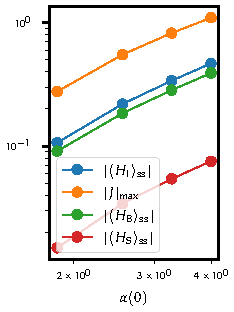
\includegraphics{figs/one_bath_syst/final_states_flows}
  \caption{\label{fig:delta_fs_flow} The absolute value difference of
    the state energies and the maximal flows for the simulations in
    \cref{fig:delta_energy_overview} from their value at coupling
    strength \(α(0)=0.40\) normalized by their value at
    \(α(0)=1.12\).}
\end{wrapfigure}
After having studied the dependence of the bath energy flow for
various cutoff frequencies of the BCF in \cref{sec:one_bath_cutoff,},
we now consider the case with fixed cutoff \(ω_c=2\) but varying
coupling strength. The results presented here are mainly a
demonstration of the feasibility of high-consistency simulations for a
range of coupling strengths. We will therefore keep the discussion of
the physical implications relatively short.

The chosen simulation parameters are the same as in
\cref{sec:one_bath_cutoff} and again consistent results have been
obtained throughout the whole range of coupling strengths as can be
gathered from \cref{fig:delta_interaction_consistency}.  The
interaction strength was chosen linearly spaced and the simulation
results are presented in \cref{fig:delta_energy_overview}.

As the shape of the BCF is not altered between the simulations, the
bath energy flows look very similar as do the interaction
energies. The main difference between the simulations is the magnitude
of the interaction energy. With increased coupling strength there is
an increased interaction energy and an increased flow which leads to
faster energy loss in the system and faster energy gain of the
bath. The stronger the coupling, the more pronounced is the
non-monotonicity in time of the interaction energy, which is reflected
in a non-monotonicity in the bath energy expectation value.

The bath energy reaches a maximum and falls slightly for the strongest
coupling simulations (violet and brown lines). If the interaction is
strong enough, ``backflow'' can occur despite finite bath correlation
times. Here, the back flow is only occurring between interaction and
bath energy. In \cref{fig:markov_analysis_steady} the bath memory is
long, additionally to a strong coupling so that multiple oscillations
can be seen.
\begin{figure}[htp]
  \centering
  \includegraphics{figs/one_bath_syst/δ_energy_overview}
  \caption{\label{fig:delta_energy_overview} Energy overview for the
    model \cref{eq:one_qubit_model} for various coupling
    strengths. The curves are converged out, and the error funnels are
    not visible.}
\end{figure}

As a task for future work it might be worthwhile to ascertain the
exact conditions under which system energy might flow back into the
system. Is resonance required and what role is played by the system
time scale? Does backflow always occur provided the coupling is strong
enough?\footnote{The author expects a negative answer to this
  question.}

Despite these differences for finite times, \cref{fig:delta_fs_flow}
demonstrates that the approximate steady state\footnote{excluding the
  \(α(0)=0.4\) case} interaction energies
\(\ev{H_{\inter}}_{\mathrm{ss}}\) (blue), maximal flows
\(\abs{J}_{\mathrm{max}}\) (orange), system energies
\(\ev{H_{\sys}}_{\mathrm{ss}}\) (red) and bath energies
\(\ev{H_{\bath}}_{\mathrm{ss}}\) (green) are almost linearly dependent
on the coupling strength \(α(0)\) in the range of coupling strengths
studied.

We find that we can control the speed of the energy transfer between
bath and system with the coupling strength at the cost of greater
steady state interaction energy. Were we to turn off the interaction
diabatically, we would have to expend this energy in the worst
case. On the other hand, more adiabatic protocol as the one used in
\cref{sec:energy-transf-char} would likely be a remedy to this
drawback.

The cooling performance for a coupling that is being turned off at the
end would depend on the concrete protocol as we've seen in
\cref{sec:one_bath_cutoff} and a more detailed study is left to future
work. The interplay between the interaction time-scale mediated by the
coupling strength, the bath memory time and the system dynamics allows
for intricate tuning.

Both the final system and bath energies are increasing with the
coupling strength, compensating for the interaction energy which is
the main mechanism that leads to residual system energy in the steady
state which is further and further away from the ground state, which
would be the steady state of weak coupling dynamics.


\fixme{iftime: re-run with same coupling strength, more cutoff freqs,
  less samples, see, longer times for coupling strengths, more coup}

\section{Conclusion}%
\label{sec:conclusion-1}

In this chapter we have validated the results of \cref{chap:flow} and
the fitness of the HOPS method for accessing bath related observables
using a direct comparison with the analytical solution of
\cref{chap:analytsol} and energy conservation in the spin-boson
model. We find that HOPS is well suited to obtain precise results
and that some trust can be placed in simulations that employ less
severe configurations, if numerical integration of the flow is
avoided. In all cases, the qualitative features of the energy
dynamics of the spin-boson model are captured very well.

We also explored the short term dynamics of the bath energy flow and
found that some light can be shed on it by considering the
approximation \(H_{\sys} = 0\). Further, the role of resonance and
bath memory time in the energy transfer performance of the zero
temperature spin-boson model was explored.

Now that we have built confidence in the method, we will turn to some
simple quantum-thermodynamical settings in
\cref{sec:therm_results}. There we will employ the capabilities of
HOPS to the fullest by treating multiple baths and (non harmonic)
modulation of the system and coupling.
